%--------------------------------------------------------------------%
% REV01: Fri 23 Jul 2021 20:08:29 WIB (RMS)
% Berkas utama templat LaTeX.
% author Petra Barus, Peb Ruswono Aryan
%--------------------------------------------------------------------%
% Berkas ini berisi struktur utama dokumen LaTeX yang akan dibuat.
%--------------------------------------------------------------------%
\documentclass[12pt, a4paper, onecolumn, oneside, final]{report}

%-------------------------------------------------------------------%
%
% Konfigurasi dokumen LaTeX untuk laporan tesis IF ITB
%
% @author Petra Novandi
%
%-------------------------------------------------------------------%
%
% Berkas asli berasal dari Steven Lolong
%
%-------------------------------------------------------------------%

% Ukuran kertas
\special{papersize=210mm,297mm}

% Setting margin
\usepackage[top=3cm,bottom=2.5cm,left=4cm,right=2.5cm]{geometry}

\usepackage{mathptmx}

% Judul bahasa Indonesia
\usepackage[bahasa]{babel}

% Format citation
%\usepackage[backend=bibtex,citestyle=authoryear]{biblatex}
\usepackage{natbib}

\usepackage[utf8]{inputenc}
\usepackage{microtype}
\usepackage{makecell}
\usepackage{graphicx}
\usepackage{csquotes}
\usepackage{tabularx}
\usepackage{listings}
\usepackage{tabto}
\usepackage{comment}
\usepackage{amsmath}
\usepackage[labelfont=bf]{caption}
\usepackage{enumitem}
\usepackage{tocbibind}
\usepackage{tocloft}
\usepackage{float}
\usepackage{indentfirst}
\usepackage[auto]{chappg}
\usepackage{titling}
\usepackage{blindtext}
\usepackage{sectsty}
\usepackage{chngcntr}
\usepackage{etoolbox}
\usepackage{hyperref}  
\usepackage{titlesec}
\usepackage{parskip}
\usepackage[htt]{hyphenat}
\usepackage{longtable}
\usepackage{pgfgantt}
\usepackage{booktabs}
\usepackage{pifont}
\usepackage{siunitx}
\usepackage[section]{placeins}
\usepackage{algorithm}
\usepackage{algpseudocode}
 
% \usepackage{ragged2e}
% \usepackage{libertine}
% \usepackage{array}
% \usepackage{textcase}
% \usepackage{setspace}
% \usepackage{afterpage}

% Line satu setengah spasi
\renewcommand{\baselinestretch}{1.5}

% Setting judul
\titlespacing*{\chapter}{0pt}{-50pt}{10pt}
\chapterfont{\centering \Large}
\titleformat{\chapter}[display]
  {\Large\centering\bfseries}
  {\chaptertitlename\ \thechapter}{0pt}
    {\Large\bfseries\uppercase}

% Setting nomor pada subbsubsubbab
\setcounter{secnumdepth}{3}
\setcounter{tocdepth}{4}

\makeatletter
\setlength{\@fptop}{0pt}
\setlength{\@fpbot}{0pt plus 1fil}
\makeatother

% Counter untuk figure dan table.
\counterwithin{figure}{chapter}
\counterwithin{table}{chapter}

% Counter untuk penomoran halaman lanjut
\newcounter{savepage}

% Kode lebih kecil
% \let\OldTexttt\texttt
% \renewcommand{\texttt}[1]{\OldTexttt{\footnotesize{#1}}}

% Pengaturan Caption
\captionsetup{labelsep=space}

% Pengaturan spasi untuk justify
\pretolerance=10000
\tolerance=2000 
\emergencystretch=10pt
%\tolerance=1
%\emergencystretch=10pt
%\hyphenpenalty=10000
%\exhyphenpenalty=1000

% Pengaturan untuk Daftar Rumus
\newcommand{\listequationsname}{Daftar Rumus}
\newlistof{myequations}{equ}{\listequationsname}
\newcommand{\myequations}[1]{%
\addcontentsline{equ}{myequations}{\protect\numberline{\theequation}#1}\par}
\setlength{\cftmyequationsnumwidth}{2.5em}

%\newcommand{\listalgorithmname}{Daftar Algoritme}
%\newlistof{algorithm}{alg}{\listalgorithmname}
%\newcommand{\algorithm}[1]{%
%\refstepcounter{algorithm}
%\par\noindent\centering\normalsize\textbf{Algoritme {\thechapter.\thealgorithm\ }\normalfont #1}
%\addcontentsline{alg}{algorithm}{\protect\numberline{\thechapter.\thealgorithm}#1}\par}
%\setlength{\cftalgorithmnumwidth}{2.5em}

% Pengaturan untuk title Daftar Isi, Tabel, dan Gambar
\renewcommand{\cfttoctitlefont}{\hspace*{\fill}\Large\bfseries\MakeUppercase}
\renewcommand{\cftaftertoctitle}{\hspace*{\fill}}
\renewcommand{\cftlottitlefont}{\hspace*{\fill}\Large\bfseries\MakeUppercase}
\renewcommand{\cftafterlottitle}{\hspace*{\fill}}
\renewcommand{\cftloftitlefont}{\hspace*{\fill}\Large\bfseries\MakeUppercase}
\renewcommand{\cftafterloftitle}{\hspace*{\fill}} 
\renewcommand{\cftequtitlefont}{\hspace*{\fill}\Large\bfseries\MakeUppercase}
\renewcommand{\cftafterequtitle}{\hspace*{\fill}} 
%\renewcommand{\cftalgtitlefont}{\hspace*{\fill}\Large\bfseries\MakeUppercase}
%\renewcommand{\cftafteralgtitle}{\hspace*{\fill}} 

\renewcommand{\cftchappresnum}{Bab }
\renewcommand{\cftchapaftersnum}{}
\renewcommand{\cftchapnumwidth}{3.7em}

\setlength{\cftbeforetoctitleskip}{-4em}
\setlength{\cftbeforeloftitleskip}{-4em}
\setlength{\cftbeforelottitleskip}{-4em}
\setlength{\cftbeforeequtitleskip}{-4em}
%\setlength{\cftbeforealgtitleskip}{-4em}

\newcolumntype{Y}{>{\centering\arraybackslash}X}

% Listing Code thingy
\lstset{frame=single,
  columns=fullflexible,
  basicstyle={\small\ttfamily},
  breaklines=true,
  breakatwhitespace=false,
  postbreak=\mbox{$\hookrightarrow$\space},
  tabsize=3
}
\renewcommand{\lstlistingname}{Kode}
\renewcommand{\lstlistlistingname}{Daftar \lstlistingname}
% \newcommand{\listingsfont}{\ttfamily}
% https://en.wikibooks.org/wiki/LaTeX/Source_Code_Listings
\renewcommand{\cftchapleader}{\cftdotfill{\cftdotsep}}

\cftsetpnumwidth{2em}


% \DefineBibliographyStrings{english}{%
%     urlseen = {Waktu akses},
%     url = {URL:},
%     and = {dan},
%     andothers = {dkk\adddot},
%     in = {dalam}
% }

% Add comma between Author and Year
%\renewcommand*{\nameyeardelim}{\addcomma\space}

% \titleformat{\paragraph}
% {\normalfont\normalsize\bfseries}{\theparagraph}{1em}{}
% \titlespacing*{\paragraph}
% {0pt}{3.25ex plus 1ex minus .2ex}{1.5ex plus .2ex}

% \titlespacing*{\section} {0pt}{2.5ex plus 1ex minus .2ex}{1.3ex plus .2ex}
% \titlespacing*{\subsection} {0pt}{2.25ex plus 1ex minus .2ex}{0.5ex plus .2ex}

% For Gantt Chart
% \newcounter{myWeekNum}
% \stepcounter{myWeekNum}
% 
% \newcommand{\myWeek}{\themyWeekNum
%     \stepcounter{myWeekNum}
%     \ifnum\themyWeekNum=53
%          \setcounter{myWeekNum}{1}
%     \else\fi
% }
% 
% \newcolumntype{L}[1]{>{\raggedright\let\newline\\\arraybackslash\hspace{0pt}}m{#1}}
% \newcolumntype{C}[1]{>{\centering\let\newline\\\arraybackslash\hspace{0pt}}m{#1}}
% \newcolumntype{R}[1]{>{\raggedleft\let\newline\\\arraybackslash\hspace{0pt}}m{#1}}
%
% \makeatletter
% \def\@chapter[#1]#2{\ifnum \c@secnumdepth >\m@ne
%                          \refstepcounter{chapter}%
%                          \typeout{\@chapapp\space\thechapter.}%
%                          \addcontentsline{toc}{chapter}%
%                                    {\protect{BAB \numberline{\thechapter}\texorpdfstring{\uppercase{#1}}{#1}}}%
%                     \else
%                       \addcontentsline{toc}{chapter}{\texorpdfstring{\uppercase{#1}}{#1}}%
%                     \fi
%                     \chaptermark{#1}%
%                     \addtocontents{lof}{\protect\addvspace{10\p@}}%
%                     \addtocontents{lot}{\protect\addvspace{10\p@}}%
%                     \if@twocolumn
%                       \@topnewpage[\@makechapterhead{#2}]%
%                     \else
%                       \@makechapterhead{#2}%
%                       \@afterheading
%                     \fi}
% \makeatother


\makeatletter

\makeatother
%\bibliography{references}
\begin{document}

%Basic configuration
\title{Pengembangan kakas untuk melakukan \textit{Performance Regression Analysis} menggunakan \textit{Distributed Tracing} pada Aplikasi berbasis Microservice}
\date{28 Maret}
\newcommand{\yearsidang}{2022}
\newcommand{\jenislaporan}{Draf Bab 4 Tugas Akhir}
\author{Rafi Abbel Mohammad}
\newcommand{\nim}{18218027}

\pagenumbering{roman}
\setcounter{page}{0}

\clearpage
\pagestyle{empty}

\begin{center}
    \smallskip

    \Large \MakeUppercase{\bfseries \thetitle}
    \vfill

    \normalsize \MakeUppercase{Laporan \jenislaporan}
    \vfill

    \normalsize Disusun sebagai syarat kelulusan tingkat sarjana
    \vfill

    \normalsize oleh:

    \normalsize \theauthor \\
    \normalsize NIM: \nim

    \vfill
    \begin{figure}[h]
        \centering
        
\includegraphics[width=0.25\textwidth]{resources/cover-ganesha.jpg}
    \end{figure}
    \vfill

    \large
    \uppercase{
        Program Studi Sistem dan Teknologi Informasi \\
        Sekolah Teknik Elektro dan Informatika \\
        Institut Teknologi Bandung
    }

    \yearsidang

\end{center}

\clearpage

\clearpage
\pagestyle{empty}

\begin{center}
    \smallskip

    \Large \bfseries \MakeUppercase{\thetitle}
    \vfill

    \Large Laporan Tugas Akhir
    \vfill

    \large Oleh

    \Large \theauthor

    \large Program Studi Teknik Informatika \\
    \normalsize \normalfont
    Sekolah Teknik Elektro dan Informatika \\
    Institut Teknologi Bandung \\

    \vfill
    \normalsize \normalfont
    Telah disetujui dan disahkan sebagai Laporan Tugas Akhir \\ di Bandung, 23 Agustus 2017 \\
    Mengetahui,

    \vfill
    \setlength{\tabcolsep}{12pt}
    \begin{tabularx}{\textwidth}{c@{\hskip 0.2\textwidth}cc@{\hskip 0.3\textwidth}}
         & {\bfseries Pembimbing}                                   & \\
         &                                                          & \\
         &                                                          & \\
         &                                                          & \\
         &                                                          & \\
         & \underline{Dr. I Gusti Bagus Baskara Nugraha S.T., M.T.} & \\
         & NIP. 19760124 201012 1 001                               &
    \end{tabularx}

\end{center}
\clearpage


\pagestyle{plain}


\titleformat*{\section}{\centering\bfseries\Large\MakeUpperCase}

\clearpage
\tableofcontents

\clearpage
{%
    \let\oldnumberline\numberline%
    \renewcommand{\numberline}{\figurename~\oldnumberline}%
    \listoffigures%
}

\clearpage
{%
    \let\oldnumberline\numberline%
    \renewcommand{\numberline}{\tablename~\oldnumberline}%
    \listoftables%
}

\clearpage
{%
    \let\oldnumberline\numberline%
    \renewcommand{\numberline}{\lstlistingname~\oldnumberline}%
    \lstlistoflistings%
}

\newpage
\setcounter{savepage}{\arabic{page}}

\titleformat*{\section}{\bfseries\large}

%----------------------------------------------------------------%
% Konfigurasi Bab
%----------------------------------------------------------------%
\renewcommand{\chaptername}{BAB}
\renewcommand{\thechapter}{\Roman{chapter}}
\pagenumbering{bychapter}
\setlength{\parindent}{1cm}
%----------------------------------------------------------------%

%----------------------------------------------------------------%
% Dafter Bab
% Untuk menambahkan daftar bab, buat berkas bab misalnya `chapter-6` di direktori `chapters`, dan masukkan ke sini.
%----------------------------------------------------------------%
\chapter{Pendahuluan}

%Pada bab ini akan dibahas mengenai gambaran dasar dari pelaksanaan Tugas Akhir dalam bentuk penjelasan latar belakang yang mendasari pemilihan topik. Dari latar belakang tersebut, akan diurai kembali menjadi rumusan masalah, tujuan, batasan masalah, metodologi, serta sistematika pembahasan tugas akhir.                                                                        
%
%\section{Latar Belakang}
%
%
%Dengan banyaknya adopsi penggunaan arsitektur Microservice yang berbasis sistem terdistribusi saat ini, semakin banyak juga tantangan yang muncul terkait dengan adopsi gaya arsitektur tersebut. Arsitektur Microservice menawarkan beberapa keuntungan antara lain heterogenitas teknologi, resiliensi, kemudahan \textit{scaling}, kemudahan \textit{deployment}, kemudahan dalam melakukan penyelarasan secara tim teknologi, fleksibilitas dalam menentukan komposisi aplikasi, dan sistem yang teroptimasi untuk melakukan penggantian kompoen satu sama lain \citep{building-microservices}. Keuntungan-keuntungan tersebut menjadikan adopsi aristektur Microservice cukup marak terutama pada aplikasi-aplikasi yang membutuhkan \textit{scalability} untuk melayani kebutuhan pelanggan yang semakin banyak.  
%
%Salah satu perusahaan yang mengadopsi arsitektur Microservice secara masif adalah Netflix \citep{netflix-nginx, netflix-infoq}. Dengan menggunakan arsitektur Microservice, para \textit{developer} di Netflix dapat melakukan dekomposisi secara \textit{decoupling} yang dapat memungkinkan \textit{developer} untuk menggunakan berbagai \textit{framework} atau bahasa pemrgoraman yang berbeda untuk setiap service nya. Hal tersebut menjadi keuntungan besar sebab para \textit{developer} dapat mendesain sebuah service dengan kemampuan dan tujuan tertentu dengan sebuah bahasa pemrograman yang sesuai dengan tujuan dari service tersebut. Kemampuan untuk melakukan hal tersebut didukung oleh teknologi \textit{container} yang dipopulerkan dengan kehadiran dari Docker dan juga teknologi \textit{container orchestration} oleh Kubernetes. Dengan adanya Kubernetes, sistem dapat melakukan \textit{scale up} dan \textit{scale down} sebuah service ketika dirasa ada \textit{workload} lebih besar yang dibutuhkan untuk mengakomodasi kebutuhan \textit{request}.
%
%Dari banyaknya keuntungan yang ditawarkan oleh arsitektur Microservice, timbul suatu permasalahan yang secara alami muncul ketika jumlah service bertambah yaitu meningkatnya kompleksitas dari sistem \citep{fowler-complexity}. Salah satu dari banyaknya kompleksitas muncul adalah dalam proses \textit{debugging}. Pada umumnya, dalam aplikasi dengan aristektur Monolith, proses \textit{debugging} hanya dilakukan pada satu sumber, sehingga jika terdapat masalah maka akan mudah ditemukan. Namun, dalam model aplkasi dengan arsitektur Microservice yang bisa memiliki ratusan bahkan ribuan service sekaligus, hal tersebut tidak akan menjadi mudah, sebab suatu \textit{bug} tertentu akan sulit dilacak jika masih menggunakan metode biasa. Hal tersebut wajar terjadi mengingat sifat terdistribusi dari service yang ada. Dari permasalahan \textit{debugging} yang terdistribusi itulah muncul suatu inisiatif untuk membuat kakas yang dapat melakukan pelacakan sistem terdistribusi atau \textit{distributed tracing} dari service-service pada suatu sistem Microservice agar para \textit{developer} dapat mendapatkan petunjuk atau \textit{observability} mengenai kondisi internal yang terjadi pada sebuah service.
%
%Sudah terdapat beberapa solusi \textit{tracing} yang ada sepanjang beberapa tahun ke belakang, dimulai dengan dipublikasikannya \textit{paper} dari Google yang mengajukan solusi \textit{tracing} untuk sistem terdistribusi bernama Dapper \citep{dapper-paper} hingga yang terbaru solusi \textit{tracing} berbasis transparan yang bernama Inkle \citep{tracing-abram}. Solusi \textit{tracing} yang diajukan Inkle berfokus untuk membuat kakas instrumentasi \textit{tracing} yang transparan, artinya proses instrumentasi tidak mengubah sama sekali kode dari sebuah service, melainkan melakukan instrumentasi data dari service dengan melakukan \textit{intercept} \textit{traffic} jaringan dari service tersebut. Metode \textit{tracing} seperti itu disebut juga dengan \textit{passive tracing}. Hasil dari metode \textit{tracing} seperti yang dilakukan Inkle adalah \textit{tracing} dapat tetap dilakukan tanpa adanya intervensi sama sekali pada level kode di dalam service, namun kekurangannya adalah akurasi hasil \textit{tracing} yang rendah dan juga hasil \textit{tracing} antar service tidak dapat menampilkan kausalitas atau hubungan sebab akibat dari \textit{request} yang dilakukan.
%
%Metode lain untuk melakukan instrumentasi pada service adalah dengan menggunakan \textit{library} pada level kode untuk memberikan konteks dan informasi kepada agen \textit{tracing}. Sudah ada beberapa \textit{library} ataupun \textit{framework} \textit{open source} yang menyediakan solusi untuk melakukan instrumentasi pada level kode seperti contohnya adalah OpenTracing, Zipkin, dan Jaeger \citep{opentracing, zipkin, jaeger}. Metode untuk melakukan tracing ini disebut juga dengan \textit{active tracing}. Dengan metode ini, data yang diperoleh dari instrumentasi akan lebih kaya, salah satunya adalah dapat memberikan konteks pemanggilan ke service lain yang nantinya dapat diolah lebih lanjut untuk mendapatkan gambaran yang lebih besar yaitu \textit{request causality} antar service.
%
%Namun dari solusi \textit{open source} yang ada, penulis menemukan adanya kekurangan dalam kakas visualisasi hasil \textit{tracing}. Penulis menemukan hanya Zipkin yang memiliki kakas visualisasi yang dapat langsung digunakan. Namun fitur visualisasi Zipkin masih berfokus pada penyediaan data \textit{tracing} dalam sebuah service dan untuk penyediaan data secara keseluruhan antar service masih belum dapat menampilkan data yang perlu untuk mencapai \textit{observability} bagi keseluruhan sistem Microservice. Dari kondisi itulah penulis menilai perlu adanya kakas yang dapat menyediakan \textit{developer} informasi yang diperlukan untuk mencapai \textit{observability} dalam sebuah sistem Microservice secara utuh. 
%
%
%\section{Rumusan Masalah}\label{RumusanMasalah}
%
%Seperti yang telah dijelaskan dalam Latar Belakang, masih adanya kekurangan dalam kakas untuk membuat visualisasi hasil \textit{distributed tracing} yang bersifat \textit{open source}. Oleh karena itu rumusan masalah yang akan dijawab pada Tugas Akhir ini adalah "Bagaimana membangun kakas solusi \textit{distributed tracing} yang dapat menampilkan visualisasi dari hasil instrumentasi \textit{tracing} pada sistem Microservice yang berjalan di atas Kubernetes?".
%
%\section{Tujuan}
%
%Tujuan yang ingin dicapai dalam Tugas Akhir ini adalah:
%\begin{enumerate}
%	\item Mengembangkan kakas solusi \textit{distributed tracing}  yang dapat menampilkan visualisasi dari hasil \textit{tracing} pada sistem Microservice yang berjalan di atas Kubernetes sehingga \textit{developer} dapat mendapatkan \textit{observability} dari sebuah sistem Microservice secara utuh
%	\item Mengukur \textit{overhead} yang diakibatkan oleh kakas solusi \textit{distributed tracing} baik pada level aplikasi maupun level infrastruktur
%\end{enumerate}
%
%
%\section{Batasan Masalah}
%
%Dalam pengerjaan Tugas Akhir ini, terdapat beberapa batasan-batasan yang perlu diperhatikan. Batasan tersebut ditujukan untuk memperjelas dan memfokuskan objek penelitian dan pengembangan tugas akhir. Batasan-batasan masalah pengerjaan tugas akhir adalah sebagai berikut,
%
%\begin{enumerate}
%	\item \textit{Library} instrumentasi yang digunakan pada level kode Microservice tidak akan dibuat dari awal namun akan mengimplementasikan \textit{library} instrumentasi \textit{open source}
%	\item Protokol komunikasi Microservice yang akan diuji terbatas pada protokol REST API, GraphQL, dan gRPC
%	\item Kasus yang diuji terbatas pada komunikasi antar aplikasi Microservice yang berjalan di atas Kubernetes
%	\item Kasus yang diuji tidak termasuk komunikasi antar aplikasi Microservice yang menggunakan protokol HTTPS
%\end{enumerate}
%
%\section{Metodologi}
%
%Metodologi yang digunakan dalam pengerjaan Tugas Akhir ini yakni:
%\begin{enumerate}
%    \item Studi Literatur \\
%          Pengerjaan tugas akhir diawali dengan mencari dan mempelajari referensi berupa buku, jurnal ilmiah dan solusi \textit{Open Source}  yang telah ada sebelumnya yang dapat membantu pengembangan kakas yang dibuat pada tugas akhir ini. Literatur yang dicari dan dipelajari berkaitan dengan topik tugas akhir yaitu mengenai \textit{Distributed Tracing},  protokol komunikasi Microservice, Kubernetes, serta hal-hal lain yang masih berkaitan dengan topik tugas akhir ini.
%
%    \item Analisis Masalah \\
%          Pada tahap ini dilakukan analisis permasalahan yang berkaitan dengan topik yang diangkat pada tugas akhir ini. Diantaranya adalah menganalisis kebutuhan instrumentasi pada protokol Microservice, kebutuhan visualisasi dari hasil \textit{tracing}, dan kebutuhan infrastruktur \textit{deployment} pada Kubernetes.
%
%    \item Perancangan Solusi \\
%          Pada tahap ini dilakukan perancangan solusi yang dapat menyelesaikan masalah-masalah yang telah dijelaskan pada bagian analisis masalah. Bagian perancangan ini juga menjelaskan arsitektur yang digunakan untuk membangun perangkat lunak berdasarkan spesifikasi dan metode yang digunakan.
%
%    \item Implementasi \\
%          Pada tahap ini dilakukan pembangunan kakas sesuai dengan kebutuhan dan spesifikasi dari hasil analisis masalah serta rancangan solusi yang diajukan.
%
%    \item Pengujian dan Analisis Hasil \\
%          Pada tahap ini dilakukan pengujian dengan menggunakan data set uji yang sesuai dengan batasan masalah ke dalam kakas yang diimplementasikan. Selanjutnya dilakukan analisis hasil pengujian dan penarikan kesimpulan.
%
%\end{enumerate}
%
%\section{Sistematika Pembahasan}
%
%Penulisan tugas akhir ini terdiri dari 5 bab, yaitu: BAB I Pendahuluan, BAB II Studi Literatur, BAB III Analisis dan Perancangan, BAB IV Rancangan, Implementasi, dan Pengujian, dan BAB V Penutup.
%
%Bab satu membahas mengenai latar belakang permasalahan, rumusan masalah, tujuan, batasan masalah, metodologi serta sistematika pembahasan yang digunakan. Bab ini juga menjelaskan secara umum isi dari tugas besar serta gambaran dasar dari pelaksanaan tugas akhir.
%
%Bab dua menjelaskan mengenai dasar teori yang digunakan di dalam menyelesaikan permasalahan yang diangkat. Teori yang digunakan berasal dari literatur dan referensi yang berhubungan dengan permasalahan yang diangkat seperti hal-hal yang berkaitan dengan \textit{Distributed Tracing}, protokol komunikasi Microservice, dan Kubernetes. Dasar teori ini menjadi dasar analisis dan rancangan solusi pada bab selanjutnya.
%
%Bab tiga memaparkan analisis permasalahan yang terkait dengan visualisasi hasil Distributed Tracing pada Microservice beserta rancangan solusi yang akan digunakan untuk mengatasi permasalahan tersebut. Selanjutnya solusi umum tersebut akan dibuat rancangan dan arsitekturnya agar dapat diimplementasikan.
%
%Bab empat memperlihatkan rancangan perangkat lunak yang dibuat serta hasil implementasinya. Pada akhir bab akan ditunjukkan hasil pengujian yang dilakukan kepada kakas yang dibuat dan pembahasan dari pengujian tersebut. Pengujian dilakukan untuk mengetahui keberhasilan kakas yang dibuat untuk menyelesaikan permasalahan yang di definisikan pada rumusan masalah.
%
%Bab lima berisikan kesimpulan terhadap hasil implementasi dan solusi yang dipaparkan untuk menyelesaikan permasalahan. Di samping itu, terdapat bagian saran yang memaparkan saran pengembangan dan perbaikan yang dapat dilakukan untuk memperkaya fitur dan menyelesaikan permasalahan yang lebih luas.
%
% \section{Jadwal Pelaksanaan}
% \newsavebox\mybox
% \begin{lrbox}{\mybox}
%     \begin{ganttchart}[
%     vgrid={*{6}{draw=none}, dotted},
%     x unit=.05cm,
%     y unit title=.6cm,
%     y unit chart=.6cm,
%     time slot format=isodate,
%     time slot format/start date=2016-09-01]{2021-09-01}{2022-04-30}
%     \ganttset{bar height=.6}
%     \gantttitlecalendar{year, month} \\
%     \ganttbar[bar/.append style={fill=blue}]{Tahap 1}{2021-09-01}{2021-11-30}\\
%     \ganttbar[bar/.append style={fill=blue}]{Tahap 2}{2021-10-01}{2021-11-15}\\
%     \ganttbar[bar/.append style={fill=blue}]{Tahap 3}{2021-11-01}{2021-12-15}\\
%     \ganttbar[bar/.append style={fill=blue}]{Tahap 4}{2021-12-15}{2022-03-01}\\
%     \ganttbar[bar/.append style={fill=blue}]{Tahap 5}{2022-02-01}{2022-04-30}
%     \end{ganttchart}
% \end{lrbox}
%
% Pengerjaan tugas akhir ini direncanakan mulai pada September 2021 sampai April 2022. Pelaksanaan tugas akhir ini dibagi menjadi 5 tahap yang dapat dipetakan kepada metodologi pengerjaan sebagai berikut,
% \begin{enumerate}
%     \item Tahap 1: Studi Literatur
%     \item Tahap 2: Analisis Masalah
%     \item Tahap 3: Perancangan Solusi
%     \item Tahap 4: Implementasi
%     \item Tahap 5: Pengujian dan Analisis Hasil
% \end{enumerate}
% Jadwal pelaksanaan tugas akhir berdasarkan metodologi pengerjaan tugas akhir dapat dilihat pada Tabel \ref{Gantt-Chart} dibawah ini.
% \begin{table}[htb]
% \centering
% \caption{Gantt Chart jadwal pelaksanaan tugas akhir}
% \label{Gantt-Chart}
% \tikz{
%   \node[inner sep=0pt,outer sep=0pt] (gantt)
%   {\begin{tabular}{c}
%     \toprule
%     \resizebox{\textwidth}{!}{\usebox\mybox} \\
%     \bottomrule
%    \end{tabular}%
%    };
% }   
% \end{table}
\chapter{Studi Literatur}

%Bab ini akan berisi pembahasan dari studi literatur yang akan berkaitan dengan permasalahan yang dibahas di Tugas Akhir ini. Hasil studi literatur akan menjadi dasar dalam pengerjaan Tugas Akhir ini baik untuk menganalisis masalah dan juga untuk merancang solusi.
%
%\section{Distributed Tracing}
%
%\subsection{\textit{Overview} Distributed Tracing}
%Dengan meningkatnya penggunaan Microservice, cara untuk melakukan \textit{profiling}, \textit{debugging}, dan \textit{monitoring} aplikasi menjadi berbeda dengan cara yang dilakukan pada aplikasi yang berbentuk Monolith.
%Salah satu cara untuk melakukan profiling pada aplikasi berbasis Microservice adalah dengan Distributed Tracing.
%Distributed Tracing, disebut juga dengan Distributed Request Tracing, adalah sebuah tipe logging terkorelasi yang dapat memberikan pengguna mendapatkan visibilitas pada operasi dari perangkat lunak terdistribusi untuk kasus seperti debugging di environment \textit{production}, dan analisis penggalian akar masalah pada kegagalan atau insiden lainnya \citep{parker2020distributed}.
%Dengan adanya kakas Distributed Tracing, pengguna dapat mendapatkan insight mengenai operasi yang terjadi di aplikasi terdistribusi secara kolektif dengan cara melakukan pelacakan pada \textit{request} yang dibuat oleh suatu \textit{service}.
%
%Kita bisa sebut setiap pekerjaan yang dilakukan oleh sebuah \textit{service} dalam suatu waktu sebagai \textit{span}.
%Setiap \textit{span} bisa diisi dengan \textit{metadata}, seringkali disebut sebagai \textit{attributes} atau \textit{tags}, dan \textit{events}, seringkali disebut sebagai \textit{logs}.
%Setiap pemanggilan Remote Procedure Call (RPC) atau Application Programming Interface (API) antara \textit{service} akan merepresentasikan hubungan dari \textit{request} yang terjadi diantara \textit{service} tersebut.
%Hubungan tersebut disebarkan diantara \textit{service} sebagai \textit{trace context}, yaitu data yang secara unik mendefinisikan \textit{span} yang dibuat oleh setiap \textit{service}.
%Setiap \textit{span} yang dibuat oleh setiap \textit{service} tersebut diteruskan kepada proses eksternal yang dapat dikumpulkan atau diagregasi sebagai sebuah \textit{trace}.
%\textit{Trace} tersebut dapat dianalisis lebih lanjut dan disimpan untuk mendapatkan \textit{insight} mengenai \textit{service}.
%Berikut adalah ilustrasi sederhana mengenai \textit{trace}:
%\begin{figure}[htb]
%      \centering
%      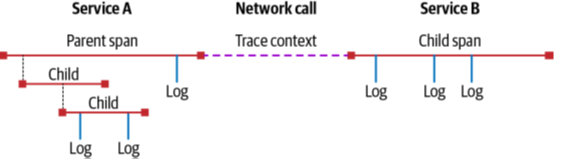
\includegraphics[width=0.6\textwidth]{resources/ch2/tracing-illus.png}
%      \caption{Ilustrasi Tracing}
%      \label{TracingIlllustration}
%\end{figure}
%
%Adapun komponen-komponen yang membangun sistem Distributed Tracing adalah sebagai berikut \citep{parker2020distributed}:
%\begin{enumerate}
%      \item Instrumentasi \\
%            Distributed Tracing membutuhkan data \textit{trace} agar dapat bekerja.
%            Data \textit{trace} dihasilkan dengan cara menginstrumentasikan proses-proses \textit{service} atau mentrasformasikan data telemetri yang sudah ada ke data \textit{trace}.
%      \item \textit{Deployment} \\
%            Setelah data \textit{trace} dihasilkan, kita perlu mengirimkan data tersebut ke suatu tempat.
%            Melakukan \textit{deployment} pada sistem \textit{tracing} membutuhkan pemahaman dimana perangkat lunak kita dijalankan di \textit{server} dan bagaimana perangkat tersebut dijalankan.
%            Agar dapat memaksimalkan kemampuan dari \textit{tracing} juga meminimalkan \textit{overhead} yang terjadi pada aplikasi, kita perlu memahami teknik yang cocok untuk melakukan deployment pada sistem Distributed Tracing yang akan kita gunakan.
%      \item Penyampaian \textit{Value} \\
%            Saat \textit{service} kita telah dapat menghasilkan data \textit{trace} dan kita telah memiliki infrastruktur yang diperlukan untuk mengolah data \textit{trace} tersebut, kita akan memerlukan kakas yang tepat untuk menggabungkan \textit{trace} dari berbagai \textit{service} dengan metadata lain seperti \textit{metrics} dan \textit{logs} untuk dapat menghasilkan \textit{value} yang berguna bagi proses \textit{debugging}, \textit{profiling}, dan \textit{monitoring} perangkat lunak terdistribusi.
%\end{enumerate}
%
%\subsection{Instrumentasi Distributed Tracing}
%
%\subsection{\textit{Deployment} Distributed Tracing}
%
%\subsection{Penyampaian \textit{Value} Distributed Tracing}
%
%\subsection{Pelacakan \textit{request causality}}
%
%\section{Protokol Komunikasi Micro\textit{service}}
%Pada subbab ini akan dijelaskan beberapa protokol komunikasi yang bisa digunakan dalam arsitektur Microsevice.
%\subsection{REST API}
%Representational State Transfer (REST) merupakan sebuah gaya arsitektur yang dibuat untuk mendesain sistem yang berjalan di World Wide Web.
%REST pertama kali diperkenalkan oleh Roy Thomas Fielding dalam disertasinya pada tahun 2005 yang berjudul \textit{Architectural Styles and the Design of Network-based Software Architectures}.
%Dalam mendesain arsitektur, REST mendefinisikan beberapa aturan yaitu skalabilitas antara komponen yang berinteraksi, antar muka yang seragam, \textit{deployment} yang independen bagi komponen, dan pembuatan arsitektur berlapis yang dapat memfasilitasi komponen untuk melakukan \textit{caching} agar dapat mengurangi \textit{latency}, memperkuat \textit{security}, dan mengenkapsulasi sistem \textit{legacy} \citep{rest}.
%
%Application Programming Interface (API) yang didesain berdasarkan prinsip-prinsip REST disebut dengan RESTful API.
%Ada dua konsep utama yang dipakai dalam mendesain REST API yaitu \textit{resources}, atau sumber daya, dan \textit{representations}, atau representasi \citep{restful-book}.
%Resource yang dimaksud dalam konteks RESTful API bisa berarti apa saja yang cukup penting untuk direferensi dan diakses sebagai API.
%Sebuah \textit{resource} biasanya sesuatu yang dapat disimpan dalam komputer seperti sebuah data yang disimpan dalam database ataupun sebuah hasil dari eksekusi algoritme.
%Satu-satunya batasan pada setiap \textit{resource} tersebut adalah setiap resource harus memiliki sebuah URL.
%Representasi sendiri menggambarkan bagaimana kondisi atau \textit{\textit{state}} saat \textit{resource} tersebut diakses.
%Contoh paling umum dari representasi  RESTful API adalah mentransportasikan \textit{resource} melalui protokol HTTP dan dalam bentuk data JSON.
%
%Dalam praktiknya, \textit{resource} sendiri tidak bisa diakses dengan sembarang cara.
%Dalam sistem RESTful API, client dan server berinteraksi dengan saling mengirim pesan yang mengikuti protokol yang sudah ditentukan sebelumnya, dalam hal ini adalah mengikuti semantik dari protokol HTTP itu sendiri.
%HTTP mendefinisikan delapan jenis pesan yang berbeda, namun ada empat yang paling sering digunakan, yaitu:
%\begin{enumerate}
%      \item GET \\
%            Dapatkan representasi dari sebuah \textit{resource}.
%      \item DELETE \\
%            Hapus \textit{resource} tersebut.
%      \item POST \\
%            Buat sebuah \textit{resource} berdasarkan representasi yang diberikan.
%      \item PUT \\
%            Gantikan \textit{state} dari \textit{resource} yang dimaksud sesuai dengan representasi yang diberikan.
%\end{enumerate}
%
%Dalam penggunaannya bagi komunikasi Microservice, RESTful API melalui HTTP masih menjadi pilihan yang paling banyak digunakan oleh developer menurut survey yang dilakukan oleh The Software House pada tahun 2020 \citep{tsh2020}.
%Walaupun adopsi nya sebagai protokol komunikasi Microservice cukup populer, namun ada beberapa kekurangan dari RESTful API \citep{web-service-article} yaitu:
%\begin{enumerate}
%      \item Tidak cocok untuk data dalam jumlah besar
%      \item Latency dan Overhead dalam pemrosesan request karena pengunaan protokol HTTP
%      \item	RESTful API memiliki ketergantungan tinggi pada Header untuk mengatur \textit{state}
%\end{enumerate}
%
%\subsection{GraphQL}
%GraphQL merupakan sebuah bahasa query dan manipulasi untuk API dan runtime untuk memenuhi query tersebut dengan data yang sudah ada \citep{graphql}.
%GraphQL dikembangkan oleh Facebook sebelum dirilis ke publik sebagai proyek Open Source pada tahun 2015.
%Pendekatan GraphQL dalam membuat API seringkali dikontraskan dengan metode pembuatan API yang sudah ada seperti REST.
%Perbedaan utama antara pendekatan GraphQL adalah cara menstrukturkan data yang diekspos ke API.
%REST melakukan penstrukturan data berdasarkan \textit{resource} sementara GraphQL menstrukturkan data lewat query yang dispesifikkan oleh pengguna seperti SQL.
%
%Sebuah layanan GraphQL dibuat dengan cara mendefinisikan tipe-tipe data pada masing-masing \textit{field}-nya kemudian menyediakan masing-masing fungsi untuk setiap \textit{field} pada tipe data tersebut.
%
%\lstinputlisting[captionpos=b, caption={Definisi Query Data}]{codes/ch2/example.graphql}
%
%\lstinputlisting[captionpos=b, caption={Fungsi Handler}]{codes/ch2/graphql-handler.js}
%
%Dari tipe data yang didefinisikan di atas, berikut adalah contoh query GraphQL beserta response-nya:
%
%\lstinputlisting[captionpos=b, caption={Query GraphQL}]{codes/ch2/query.graphql}
%
%\lstinputlisting[captionpos=b, caption={\textit{Response} GraphQL dalam JSON}]{codes/ch2/response.json}
%
%\subsection{gRPC}
%gRPC adalah sebuah \textit{framework} Remote Procedure Call (RPC) Open Source berperforma tinggi yang dapat dijalankan di berbagai environment (gRPC Authors 2021).
%gRPC dapat secara efisien menghubungkan \textit{service} yang berada di dalam dan antara data center dengan berbagai dukungan untuk melakukan load balancing, tracing, pengecekan kesehatan, dan autentikasi.
%gRPC juga dapat diaplikasikan pada server yang terdistribusi untuk menghubungkan berbagai perangkat mulai dari aplikasi mobile dan browser ke layanan backend.
%Seperti RPC pada umumnya, gRPC memungkinkan \textit{service} yang terpisah untuk mengakses fungsi layaknya objek lokal. Ada beberapa skenario penggunaan utama dari gRPC:
%\begin{enumerate}
%      \item Menghubungkan service-service yang bersifat poliglot seperti dalam arsitektur Microservice.
%      \item Menghubungkan perangkat mobile, browser client ke service backend.
%      \item Menghasilkan library bagi sisi client yang efisien.
%\end{enumerate}
%
%Secara default, gRPC menggunakan Protocol Buffers sebagai Interface Definition Language (IDL) dan juga sebagai format pertukaran pesannya (walaupun juga bisa menggunakan JSON sebagai format pertukaran data).
%Langkah pertama ketika menggunakan Protocol Buffers adalah dengan mendefinisikan struktur dari data yang ingin diserialisasi dalam sebuah file proto, yaitu sebuah file teks biasa yang memiliki ekstensi “.proto”.
%Data dari Protocol Buffers distrukturkan sebagai messages yang masing-masing memiliki catatan mengenai data yang berbentuk pasangan name-value yang disebut dengan fields.
%Berikut adalah contoh sederhana dari file proto:
%\lstinputlisting[captionpos=b, caption={Contoh File Proto}]{codes/ch2/hello.proto}
%
%Ketika struktur data sudah dibuat, kode Proto tersebut perlu di compile menggunakan kakas bernama protoc yang akan membuat akses data dalam bahsa pemrograman yang dipilih.
%gRPC menggunakan protoc untuk menghasilkan kode dari file Proto berupa: kode gRPC bagi client dan server, dan juga kode Protocol Buffer biasa yang digunakan untuk melakukan populasi, serialisasi, dan kode untuk mendapatkan tipe pesan.
%
%Adapun penggunaan gRPC pada sistem client dan server adalah sebagai berikut:
%\begin{enumerate}
%      \item Mendefinisikan service beserta method apa saja yang bisa dipanggil beserta parameter dan juga return type bagi masing-masing method.
%      \item  Server akan mengimplementasi interface hasil kompilasi protoc yang berasal dari method-method yang didefinisikan pada file proto.
%      \item Client akan memanggil method yang sudah didefinisikan pada server.
%\end{enumerate}
%
%\subsection{WebSocket}
%
%
%\section{Kubernetes}
%\subsection{Arsitektur Kubernetes}
%Arsitektur Kubernetes terdiri atas dua macam node yaitu master node dan worker node.
%Setiap cluster Kubernetes terdiri dari minimal satu buah worker node dan satu atau lebih worker node.
%Master node akan mengatur semua worker node dan pod yang ada di dalam cluster.
%Dalam environment production, biasanya master node akan berjalan di beberapa komputer dan cluster akan berjalan dengan beberapa node sehingga menyediakan sifat fault-tolerance dan high-availability \citep{kube-arch}.
%Untuk mengakses cluster Kubernetes, pengguna akan menspesifikkan perintah kepada master node melalui aplikasi command line bernama kubectl dan master node akan menyesuaikan state yang diminta oleh pengguna dengan memberikan perintah kepada worker node yang tersedia seperti membuat pod baru.
%Berikut adalah gambaran arsitektur Kubernetes:
%\begin{figure}[htb]
%      \centering
%      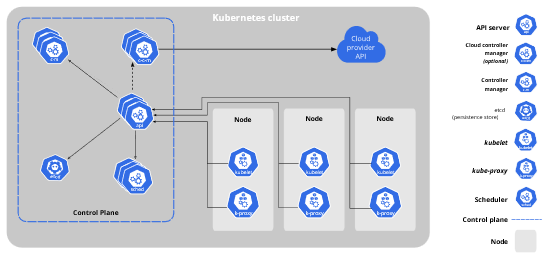
\includegraphics[width=0.9\textwidth]{resources/ch2/kube-1.png}
%      \caption{Arsitektur Kubernetes \citep{kube-arch}}
%      \label{KubeArch}
%\end{figure}
%
%Adapun komponen-komponen yang terdapat pada master node antara lain:
%\begin{enumerate}
%      \item Kube-apiserver adalah komponen dari master node yang mengekspos API Kubernetes. API Server adalah frontend dari worker node / control plane bagi Kubernetes.
%      \item Etcd adalah komponen yang berfungsi sebagai penyimpan data yang konsisten dan higly-available dengan skema penyimpanan key-value.
%      \item	Kube-scheduler berfungsi sebagai pengawas dan penjadwal bagi pod yang baru dibuat dan tugasnya adalah untuk menetapkan dimana node  bagi pod tersebut.
%      \item	Kube-controller-manager adalah komponen yang berfungsi untuk menjalankan proses controller yaitu fungsi yang bertanggung jawab mengelola pod, worker node, dan mengatur tugas jika terjadi kegagalan pada proses pembuatan pod.
%\end{enumerate}
%
%Adapun komponen-komponen yang terdapat pada worker node antara lain:
%\begin{enumerate}
%      \item  Kubelet adalah komponen yang berfungsi sebagai agen di setiap node yang ada pada cluster dan bertugas untuk memastikan container yang berjalan pada pod.
%      \item Kube-proxy adalah sebuah proxy jaringan yang berjalan di setiap node pada cluster dan mengimplementasikan konsep dari service Kubernetes.
%      \item Container Runtime adalah sebuah perangkat lunak yang bertanggung jawab untuk menjalankan container. Kubernetes sendiri mendukung beberapa Container Runtime seperti Docker, containerd, CRI-O, dan semua jenis Runtime yang mengimplementasi Kubernetes CRI (Container Runtime Interface).
%\end{enumerate}
%
%\subsection{Pod}
%Pod adalah unit terkecil yang dapat di deploy di dalam sebuah Kubernetes cluster.
%Pod sendiri adalah sebuah abstraksi dari container yang di deploy di Kubernetes.
%Jadi, ketika seorang pengguna ingin membuat sebuah aplikasi berbasis container di Kubernetes, pengguna tidak melakukan deploy container secara langsung melainkan melalui object Kubernetes yang bernama Pod.
%Di dalam Pod sendiri bisa terdapat lebih dari satu buah container sekaligus sesuai dengan kebutuhan.
%Contohnya ada jenis container yang disebut sebagai sidecar yang berfungsi sebagai secondary unit dari container utama yang ada di dalam Pod tersebut.
%\subsection{Controller}
%Kita bisa langsung membuat Pod di kubernetes lewat command line interface.
%Namun jika kita membuat secara manual Pod, maka kita juga harus bertanggung jawab selama lifecycle dari Pod tersebut.
%Masalah timbul ketika kita ingin membuat beberapa Pod yang sama sekaligus, maka akan menjadi suatu tugas yang tidak mudah untuk mengatur Pod-Pod tersebut.
%Dari permasalahan itulah, ada sebuah konsep di Kubernetes yang disebut dengan Controller.
%
%Controller adalah sebuah abstraksi di atas Pod yang bertugas untuk mengelola Pod secara otomatis dengan memanfaatkan komponen di dalam Pod yang bernama Container Probes.
%Container Probes akan berfungsi untuk melakukan pengecekan apakah container yang berada di Pod berjalan dengan baik.
%Jika Container Probes memberi tahu Controller bahwa container tidak berjalan dengan baik, maka Controller akan melakukan reset pada container tersebut.
%
%Pada implementasinya, Kubernetes memiliki dua jenis implementasi dari Controller yaitu ReplicaSet dan DaemonSet.
%
%\subsection{ReplicaSet}
%ReplicaSet adalah jenis Controller yang bertanggung jawab untuk mengelola kebutuhan Pod sesuai state yang dispesifikkan oleh pengguna.
%Cara ReplicaSet melakukan monitor pada Pod adalah melalui label yang telah ditetapkan ke sebuah Pod.
%Jika label tersebut dengan selector yang terdapat pada ReplicaSet maka Pod akan masuk ke pengawasan dari ReplicaSet.
%ReplicaSet akan mencocokkan keadaan Pod dengan spesifikasi yang diberikan oleh pengguna sehingga ketika ReplicaSet melihat bahwa Pod tidak sesuai dengan spesifikasi, contohnya banyaknya Pod tidak sesuai, ataupun satu node mati sehingga Pod yang ada di dalamnya terdampak, maka ReplicaSet akan menyesuaikan kondisi Pod tersebut.
%
%\subsection{DaemonSet}
%DaemonSet adalah jenis Controller yang memiliki fungsi untuk mengatur agar tepat ada satu Pod pada setiap node.
%DaemonSet biasanya digunakan untuk mengelola Pod yang erat fungsinya dengan infrastruktur dari Kubernetes seperti mengatur jalannya operasi sistem, mengumpulkan log, atau memonitor resource di setiap node.
%
%\subsection{Deployment}
%Deployment adalah suatu abstraksi Controller di atas ReplicaSet yang tugasnya adalah melakukan deployment aplikasi Container di Kubernetes.
%Deployment akan bekerja dengan mengatur ReplicaSet yang ada untuk mengatur pembaruan yang terjadi pada sebuah versi aplikasi Deployment.
%Cara yang dilakukan oleh Deployment dalam mengatur versi aplikasi adalah dengan mengontrol ReplicaSet yang mengatur Pod.
%Jika kita melakukan upgrade sebuah aplikasi pada Deployment, pertama kali Deployment akan menginstruksikan kepada ReplicaSet untuk mengurangi jumlah Pod yang diatur hingga nol.
%Baru kemudian Deployment menginstruksikan kembali ReplicaSet untuk membuat Pod sebanyak spesifikasi.
%
%Dengan fitur semacam itu, Deployment dapat memberikan fungsionalitas update tanpa adanya down time seperti melakukan rollback jika versi Deployment yang baru tidak sesuai yang diinginkan oleh pengguna.
%
%\subsection{Service}
%Fungsi networking adalah salah satu yang terpenting dalam sebuah sistem terdistribusi sebab suatu komponen perlu untuk berkomunikasi dengan komponen lainnya, dalam hal ini Pod.
%Seperti yang sudah dipaparkan sebelumnya, Pod akan dikontrol oleh Controller, dalam hal ini adalah ReplicaSet melalui Deployment.
%Dari sistem itu, ada kemungkinan bahwa Pod ynag berisi sebuah aplikasi container akan berubah sesuai yang dikehendaki oleh Controller-nya.
%Jika kita melakukan komunikasi antar Pod langsung melalui IP address dari Pod tersebut, maka jika Pod tersebut hilang atau digantikan oleh Controller-nya maka IP address yang lama akan tidak bisa digunakan kembali.
%
%Untuk menyelesaikan permasalahan tersebut, Kubernetes menggunakan sebuah layer abstraksi untuk Networking yang dinamakan Service.
%Service akan menyediakan entry kepada sebuah Pod melalui Controller-nya, yaitu Deployment dan Service akan menyediakan IP address dan juga DNS entry yang tetap sehingga ketika Pod di dalam Deployment tersebut berubah, Pod akan tetap bisa diakses melalui Service.
%
%Untuk memudahkan discovery dari sebuah Service, kubernetes memiliki sistem DNS nya sendiri yang diatur melalui master node.
%Cara mengakses nya secara standar adalah jika pada sebuah Namespace yang sama, komponen Kubernetes yang lain dapat mengakses Service dan port nya langsung dengan format nama service itu sendiri.
%Namun jika sebuah komponen Kubernetes lainnya mengakses Service tersebut dari luar Namespace tempat Service di deploy, maka cara pengaksesannya mengikuti format seperti berikut: \textit{[nama service].[namespace].svc.cluster.local}.
%
%Dalam mengakomodasikan kebutuhan networking di Kubernetes, Service sendiri memiliki beberapa jenis yang dapat digunakan untuk berbagai usecase yang berbeda.
%Tipe-tipe Service tersebut adalah:
%\begin{enumerate}
%      \item ClusterIP \\
%            ClusterIP adalah tipe default dari Service. Seperti namanya, ClusterIP akan berbentuk sebuah IP address yang hanya bisa diakses dari dalam cluster dengan DNS.
%      \item NodePort \\
%            Dengan tipe Service ini, Kubernetes akan membuat sebuah port yang sama pada semua node yang dapat diakses dari luar cluster.
%      \item LoadBalancer \\
%            Tipe LoadBalancer adalah tipe Service khusus yang dipergunakan untuk mengekspos Service ke luar cluster melalui sebuah layanan Load Balancer. Layan Load Balancer yang dapat dipergunakan sendiri bisa dipilih sesuai dengan dimana cluster Kubernetes dibuat. Jika cluster dibuat di salah satu penyedia jasa Cloud Computing, maka LoadBalancer akan menggunakan layanan Load Balancer dari Cloud Computing tersebut untuk mengekspos Service ke luar cluster.
%\end{enumerate}
%
%
%\section{Penelitian Terkait}
\chapter{Analisis Masalah dan Perancangan Solusi}
%Pada bab ini diuraikan analisis persoalan \textit{Performance Regression Analysis} yang telah diuraikan pada Bab I. Hasil dari bab ini digunakan untuk merancang kakas yang akan diimplementasikan seperti yang dijelaskan pada Bab IV. 
%
%
%\section{Analisis Masalah}
%\label{analisis-masalah}
%
%Seiring dengan meningkatnya kompleksitas dari aplikasi Microservice, seperti dengan meningkatnya jumlah service dan keterhubungan antar service yang ada di dalamnya, akan meningkat juga kompleksitas untuk melakukan \textit{monitoring} terhadap kinerja pada keseluruhan aplikasi Microservice. Salah satu isu penting terkait dengan kinerja adalah regresi atau penurunan terhadap kinerja. Kebutuhan untuk dengan segera menentukan penyebab utama dari regresi pada sistem menjadi penting apabila regresi terjadi pada lingkungan produksi yang langsung melayani \textit{request} dari pelanggan, sehingga apabila tidak diatasi dengan segera akan berdampak langsung terhadap pengalaman pengguna dalam menggunakan aplikasi. 
%
%Terdapat dua pendekatan yang dapat dilakukan untuk mengatasi permasalahan regresi kinerja \citep{regression-detection}, yaitu:
%\begin{enumerate}
%	\item Deteksi regresi dilakukan setelah aplikasi selesai dikembangkan dan di-\textit{deploy} pada lingkungan terdedikasi
%	\item Deteksi regresi dilakukan sebelum aplikasi selesai dikembangkan dan di-\textit{deploy} dan melakukan studi terhadap perubahan yang dihasilkan pada \textit{source code}
%\end{enumerate}  
%
%Mengingat sifat dari Microservice yang terdistribusi, akan menjadi sulit bagi \textit{developer} jika pendeteksian regresi dilakukan dengan pendekatan individual pada masing-masing service yang ada terlebih ketika jumlah service yang ada sudah sangat banyak dan hubungan interdependensi antar service menjadi rumit. Oleh karena itu, untuk mengatasi regresi kinerja pada aplikasi berbasis Microservice, dibutuhkanlah pendekatan yang tidak mengharuskan \textit{developer} untuk melakukan pencarian sumber masalah pada masing-masing service secara individu. Sehingga pada kasus deteksi dan analisis regresi kinerja aplikasi berbasis Microservice, pendekatan pertama lebih cocok untuk digunakan.
%
%Salah satu teknologi yang dapat digunakan untuk melakukan \textit{monitoring} dan analisis regresi pada sebuah sistem terdistribusi seperti Microservice adalah \textit{distributed tracing}. Dengan bantuan mekanisme \textit{span} dari \textit{trace}, metrik-metrik kinerja dalam aplikasi berbasis Microservice dapat dilacak secara menyeluruh. Dalam kasus penggunaan seperti yang telah disebutkan sebelumnya, \textit{distributed tracing} cocok untuk digunakan dalam melakukan analisis regresi kinerja atau \textit{Performance Regression Analysis} dalam sebuah aplikasi berbasis Microservice sebab \textit{developer} tidak perlu menganalisis satu per satu \textit{service} yang ada terutama setelah \textit{service} sudah di-\textit{deploy}.
%
%Oleh karena itu, dapat dirumuskan alur kerja yang harus dilakukan oleh sistem \textit{Performance Regression Analysis} (PRA) sebagai berikut:
%\begin{enumerate}
%	\item Sistem harus dapat mendeteksi ketika terjadi regresi pada aplikasi berbasis Microservice
%	\item Sistem harus dapat menentukan sumber atau akar permasalahan dari regresi setelah terdeteksi
%\end{enumerate}
%
%Sudah terdapat beberapa pendekatan yang dapat digunakan untuk melakukan analisis regresi seperti yang ada pada subbab \ref{ch2-algo}. Melihat kebutuhan dari sistem PRA di atas, dari beberapa pendekatan yang ada pada subbab tersebut, penulis menilai ada dua pendekatan yang dapat digunakan yaitu pendekatan Analisis Kumulatif pada \ref{approach-cumulative} dan pendekatan Analisis Agregasi dan Korelasi pada \ref{approach-corr}. Analisis Kumulatif dapat digunakan untuk menentukan apakah telah terjadi regresi pada aplikasi dengan melakukan perbandingan antara CDF \textit{baseline} dengan CDF dari aplikasi yang sedang berjalan. Ketika didapatkan statistik K-S yang melebihi \textit{threshold}, sistem PRA akan melakukan analisis akar permasalahan dengan metode Analisis Agregasi dan Korelasi untuk mendapatkan penyebab dari regresi melalui analisis \textit{crtical path} pada \textit{service} yang terdeteksi memiliki koefisien korelasi tinggi. Penghitungan koefisien korelasi dapat dilakukan dengan menghitung koefisien korelasi antara hasil \textit{trace} ketika terdeteksi regresi dengan hasil \textit{trace} dari \textit{baseline}.
%
%Gambar \ref{alur-pra} menggambarkan fase yang akan dilakukan oleh sistem PRA. Secara umum, akan terdapat dua fase yang akan dilakukan yaitu fase \textit{baseline loading phase} dan fase \textit{realtime analysis phase}. Fase pertama yaitu \textit{loading phase} akan mencari data dari aktivitas aplikasi yang bersifat stabil yang dapat digunakan sebagai \textit{baseline} atau acuan bagi analisis yang akan dilakukan pada tahap-tahap selanjutnya. Fase ini akan menghasilkan tiga buah artifak yaitu fungsi \textit{cumulative distribution function} (CDF) dari histogram hasil \textit{trace}; sampel \textit{trace} yang mencakup seluruh fitur yang ada seperti \textit{service}, operasi, \textit{tag}, \textit{error} beserta masing-masing data durasi \textit{span} yang dapat disimpan sebagai pasangan \textit{key-value}; dan data operasi yang terjadi pada \textit{critical path} semua \textit{span} beserta nilai \textit{latency}-nya yang akan disimpan juga sebagai pasangan \textit{key-value}. 
%
%Fase berikutnya adalah fase analisis secara \textit{realtime}. Ada beberapa tahap analisis yang akan dilakukan pada fase ini.  Tahap analisi pertama akan membandingkan hasil transformasi CDF histogram \textit{tracing} yang sedang berlangsung secara \textit{realtime} dengan CDF \textit{baseline} hasil fase \textit{loading}. Perbandingan tersebut akan dilakukan dalam periode tertentu. Perbandingan dari kedua CDF tadi akan menghasilkan statistik Kolmogorov-Smirnov (K-S). Jika statistik K-S yang dihasilkan melebihi batas \textit{threshold} \textit{significance level} dari statistik K-S, maka dapat disimpulkan bahwa terjadi regresi pada periode \textit{capture} histogram tersebut. 
%
%Jika terdeteksi terjadi regresi, tahap selanjutnya adalah melakukan analisis korelasi seperti yang telah dijelaskan pada \ref{approach-corr}. Sampel perbandingan \textit{trace} yang akan digunakan adalah sampel \textit{trace} yang berasal dari data sampel \textit{baseline}. Hasil korelasi kemudian diurutkan dan akan dicek selanjutnya mana saja fitur seperti \textit{service} yang nilai koefisien korelasinya melebihi \textit{threshold} batas korelasi. Kemudian selanjutnya akan dihitung nilai kontribusi \textit{critical path} pada \textit{service} yang terindikasi mengalami regresi dan hasil perhitungan kontribusi \textit{latency} dari \textit{critical path} tersebut akan dibandingkan dengan data \textit{latency} \textit{critical path} yang berasal dari perhitungan \textit{baseline}. Dari perbandingan tadi, akan diurutkan dan didapatlah hasil operasi mana yang memiliki perubahan \textit{latency} terbesar dan menjadi kandidat kuat sebagai akar permasalahan penyebab regresi.
%
%\begin{figure}[!htb]
%	\centering
%	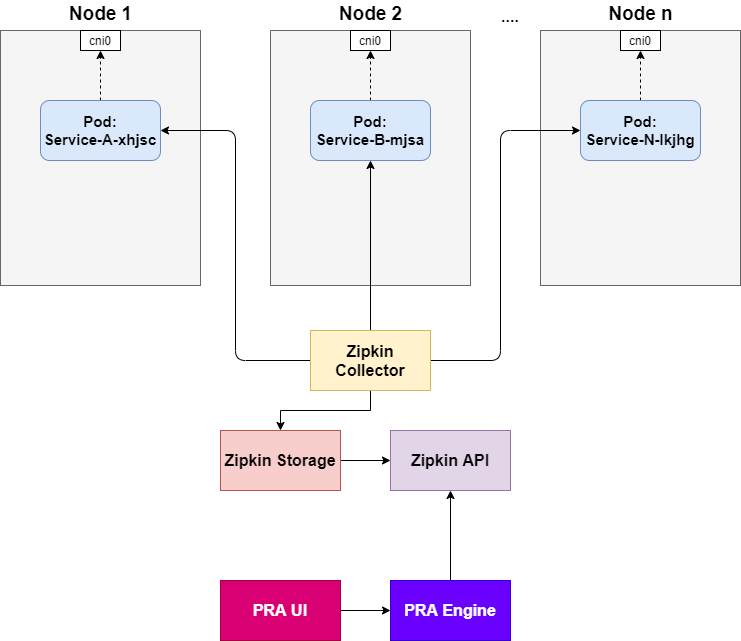
\includegraphics[width=1\textwidth]{resources/ch3/alur.png}
%	\caption{Alur sistem \textit{Performance Regression Analysis}}
%	\label{alur-pra}
%\end{figure}
%
%\section{Rancangan Solusi}
%
%\subsection{Pemilihan Solusi \textit{tracing}}
%
%Dari pemaparan alur sistem \textit{Performance Regression Analysis} pada subbab \ref{analisis-masalah}, dapat dirumuskan beberapa kriteria sistem \textit{distributed tracing} yang akan digunakan. Daftar kriteria dapat dilihat pada Tabel \ref{ch3-trace-crit}.
%
%Dari berbagai jenis solusi \textit{distributed tracing} yang sudah ada seperti pada subbab \ref{terkait}, penulis menilai Zipkin merupakan solusi yang tepat untuk digunakan sebab memenuhi semua kriteria pada tabel di atas. Untuk kriteria TC-1, Zipkin menggunakan metode instrumentasi secara \textit{active} dengan menambahkan informasi header \textit{span} induk dan \textit{span} anak pada setiap \textit{request} sehingga hubungan kausalitas antar \textit{service} dalam \textit{request} dapat dicatat sebagai hubungan induk-anak dalam \textit{span}. Untuk kriteria TC-2, sudah terdapat dukungan untuk membuat \textit{deployment} di Kubernetes dari komunitas \textit{Open Source} \citep{zipkin-ambassador}. Untuk kriteria TC-3, Zipkin menyediakan dukungan ekstensi bagi komponen \textit{collector} dan \textit{storage} dari pihak ketiga dan sudah didukung secara \textit{native} untuk beberapa komponen \citep{zipkin-storage}.
%
%\begin{small}
%	\begin{longtable}{ | p{3cm} | p{10cm} |}
%		\caption{Kriteria pemilihan solusi \textit{tracing}}
%		\label{ch3-trace-crit}                                                           
%		\\ \hline
%		\centering\bfseries{ID Kriteria} & \centering\bfseries{Deskripsi} \tabularnewline \hline
%		\endfirsthead
%		TC-1 & Komponen instrumentasi dapat menyediakan informasi kausalitas antar \textit{service} yang terjadi selama \textit{request} pada \textit{span} \\ \hline
%		TC-2 & Komponen \textit{deployment} menyediakan dukungan untuk Kubernetes \\ \hline
%		TC-3 & Komponen \textit{deplyoment} menyediakan dukungan untuk \textit{storage} eksternal \\ \hline
%	\end{longtable}
%\end{small}
%
%\subsection{Arsitektur Solusi}
%
%Gambar \ref{arch-pra} menunjukkan arsitektur dari solusi \textit{distributed tracing} yang akan digunakan untuk melakukan \textit{Performance Regression Analysis}. Komponen utama \textit{tracing} yang akan digunakan sesuai dengan arsitektur \textit{tracing} yang dimiliki oleh Zipkin seperti pada gambar \ref{zipkin-arch}. Komponen instrumentasi akan menggunakan \textit{library} \textit{tracing} milik Zipkin dan akan ditempatkan pada level kode pada setiap \textit{service}. Sementara itu \textit{collector} Zipkin akan di-\textit{deploy} sebagai DaemonSet untuk mengakomodasi sifat terdistribusi dari Kubernetes. Sehingga setiap \textit{service} yang di-\textit{deploy} sebagai Pod akan melakukan \textit{transport} data \textit{span} melalui HTTP kepada \textit{collector} yang berada pada Node yang sama via DaemonSet. Komponen \textit{storage} dan API masing-masing akan dideploy menggunakan Deployment dan berfungsi untuk mengumpulkan data dari \textit{collector}. Sistem PRA akan dibuat terpisah menjadi dua komponen yaitu komponen Engine dan juga User Interface (UI). Komponen Engine akan berfungsi untuk mengimplementasikan logika dari sistem PRA sesuai dengan alur kerja pada gambar \ref{alur-pra}. Engine akan mengekspos data yang telah diolah lewat gRPC. Komponen UI akan berfungsi untuk menampilkan data \textit{trace} dan juga menampilkan hasil kerja proses PRA yang datanya bersumer dari komponen Engine. UI akan mengambil beberapa komponen dari UI standard Zipkin dan menambahkan fungsionalitas sesuai dengan alur kerja sistem PRA.
%
%\begin{figure}[!htb]
%	\centering
%	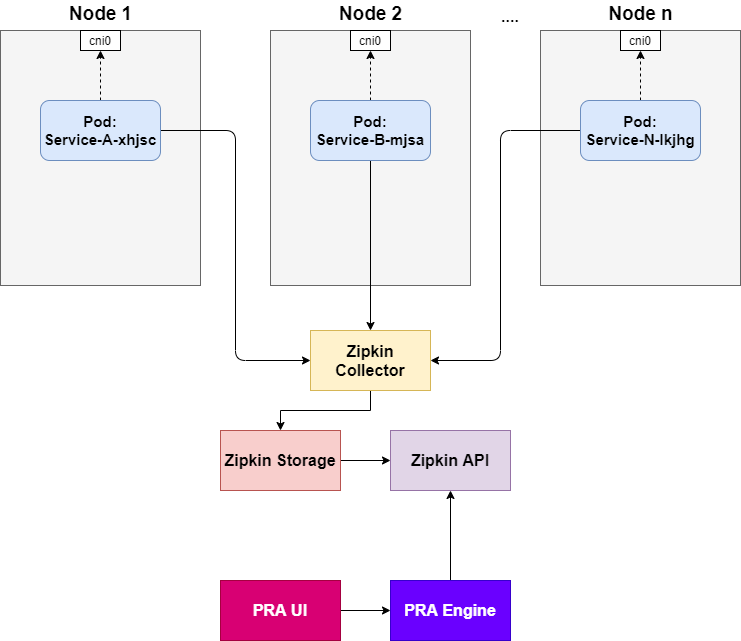
\includegraphics[width=1\textwidth]{resources/ch3/arch.png}
%	\caption{Arsitektur sistem \textit{Performance Regression Analysis}}
%	\label{arch-pra}
%\end{figure}
%
%\section{Jadwal Pelaksanaan}
% 
% \newsavebox\mybox
% \begin{lrbox}{\mybox}
%	     \begin{ganttchart}[
%		     vgrid={*{6}{draw=none}, dotted},
%		     x unit=.05cm,
%		     y unit title=.6cm,
%		     y unit chart=.6cm,
%		     time slot format=isodate,
%		     time slot format/start date=2016-09-01]{2021-09-01}{2022-04-30}
%		     \ganttset{bar height=.6}
%		     \gantttitlecalendar{year, month} \\
%		     \ganttbar[bar/.append style={fill=blue}]{Studi Literatur}{2021-09-01}{2021-11-30}\\
%		     \ganttbar[bar/.append style={fill=blue}]{Analisis Masalah}{2021-10-01}{2021-11-15}\\
%		     \ganttbar[bar/.append style={fill=blue}]{Perancangan Solusi}{2021-11-01}{2021-12-15}\\
%		     \ganttbar[bar/.append style={fill=blue}]{Implementasi}{2021-12-15}{2022-03-01}\\
%		     \ganttbar[bar/.append style={fill=blue}]{Pengujian dan Analisis Hasil}{2022-02-01}{2022-04-30}
%		     \end{ganttchart}
%	 \end{lrbox}
%
% Pengerjaan tugas akhir ini direncanakan mulai pada September 2021 sampai April 2022. Pelaksanaan tugas akhir ini dibagi menjadi 5 tahap yang dapat dipetakan kepada metodologi pengerjaan sebagai berikut,
% \begin{enumerate}
%	     \item Tahap 1: Studi Literatur
%	     \item Tahap 2: Analisis Masalah
%	     \item Tahap 3: Perancangan Solusi
%	     \item Tahap 4: Implementasi
%	     \item Tahap 5: Pengujian dan Analisis Hasil
%	 \end{enumerate}
% 
% Jadwal pelaksanaan tugas akhir berdasarkan metodologi pengerjaan tugas akhir dapat dilihat pada Tabel \ref{Gantt-Chart} dibawah ini.
% \begin{table}[htb]
%	 \centering
%	 \caption{Gantt Chart jadwal pelaksanaan tugas akhir}
%	 \label{Gantt-Chart}
%	 \tikz{
%		   \node[inner sep=0pt,outer sep=0pt] (gantt)
%		   {\begin{tabular}{c}
%				     \toprule
%				     \resizebox{\textwidth}{!}{\usebox\mybox} \\
%				     \bottomrule
%				    \end{tabular}%
%			    };
%		 }   
%	 \end{table}
%
%
%

\chapter{Implementasi dan Pengujian}

Bab ini akan membahas seluruh proses implementasi yang dilakukan untuk menerapkan rancangan yang sudah didefinisikan sebelumnya. Selain itu, bab ini juga akan membahas pengujian yang dilakukan terhadap hasil implementasi yang mencakup hal-hal yang diuji, metode pengujian, dan hasil pengujian yang diperoleh. 


\section{Implementasi}
Implementasi sistem \textit{Performance Regression Analysis} (PRA) akan dibuat berdasarkan rancangan arsitektur seperti yang terdapat pada gambar \ref{arch-pra}. Komponen seperti \textit{library} instrumentasi, melainkan akan melakukan \textit{fork} dan modifikasi solusi \textit{Open Source} \textit{distributed tracing} dari Zipkin. Komponen yang akan dibuat dari awal sepenuhnya adalah komponen PRA \textit{User Interface} (UI) dan PRA Engine dari sistem PRA yang akan melakukan komputasi utama sistem pendeteksian dan analisis regresi. Komponen PRA Engine juga akan berfungsi sebagai API yang akan diakses oleh komponen PRA UI.



\subsection{Implementasi PRA Engine}

Sebelum melakukan implementasi solusi, penulis harus terlebih dahulu melakukan pemilihan kakas yang akan digunakan melakukan implementasinya. Secara umum, terdapat banyak bahasa pemrograman yang dapat melakukan implementasi solusi komponeasdn \textit{engine} sesuai dengan alur yang terdapat pada gambar \ref{alur-pra}. Namun, ada suatu kebutuhan penting untuk melakukan tes statistik Kolmogorov-Smirnov (K-S) yang tidak semua bahasa pemrograman memiliki dukungan \textit{library} untuk melakukannya. Terdapat dua bahasa pemrograman yang memiliki \textit{library} untuk melakukan tes K-S yaitu bahasa pemrograman \textbf{Go} dan \textbf{Python}. Bahasa \textbf{Go} memiliki library Gonum \footnote{\url{gonum.org}} yang memiliki implementasi tes K-S dalam fungsi \texttt{KolmogorovSmirnov}, sementara bahasa \textbf{Python} memiliki library SciPy \footnote{\url{scipy.org}} yang memiliki implementasi tes K-S dalam fungsi \texttt{scipy.stat.ks\textunderscore 2samp}.

Dari kedua bahasa tersebut, penulis memilih bahasa \textbf{Python} untuk melakukan implementasi solusi setelah berhasil melakukan \textit{parsing} data \textit{trace} Zipkin dengan pendekatan pemrograman berorientasi objek yang didasarkan pada \textit{source code} yang dimiliki oleh aplikasi \textit{User Interface} milik Zipkin yang diimplementasikan menggunakan bahasa \textbf{Javascript}. 

Implementasi \textit{engine} akan terbagi menjadi beberapa modul seperti yang terlihat pada tabel \ref{engine-module}.

\begin{small}
	\begin{longtable}{ | p{1cm} | p{3cm} | p{10cm} | }
		\caption{Tabel pembagian modul komponen \textit{engine}}
		\label{engine-module}                                                           
		\\ \hline
		\centering\bfseries{ID} & \centering\bfseries{Nama Modul} & \centering\bfseries{Deskripsi} \tabularnewline \hline
		\endfirsthead
		EM-1 & zipkin (Pengambilan Data) & Modul ini bertanggung jawab untuk mengambil data dari API Zipkin yang memiliki data hasil \textit{trace} dari aplikasi. \\ \hline
		EM-2 & transform (Transformasi Data) & Modul ini bertanggung jawab untuk melakukan transformasi dari data \textit{trace} mentah yang diambil dari API Zipkin menjadi bentuk-bentuk model yang akan digunakan untuk komputasi di tahap selanjutnya seperti sampel data \textit{latency}, dan model data \textit{Critical Path}. Semua model akan disimpan dalam data berbentuk JSON. \\ \hline
		EM-3 & storage (Penyimpanan Data) & Modul ini bertanggung jawab untuk menyimpan model hasil transformasi \textit{baseline} dari modul EM-2 ke \textit{storage} untuk digunakan kembali pada fase \textit{Periodical Analysis}. Komponen \textit{storage} yang akan digunakan adalah Redis. Alasan utama pemilihan Redis sebagai komponen \textit{storage} adalah Redis telah memiliki modul penyimpanan data dalam bentuk JSON dan memiliki kinerja yang tinggi sebab data disimpan secara \textit{in-memory}. \\ \hline
		EM-4 & statistic (Perhitungan Statistik) & Modul ini bertanggung jawab untuk melakukan komputasi perhitungan statistik yang mencakup pendeteksian regresi dengan menghitung koefisien Kolmogorov-Smirnov seperti yang telah dijelaskan pada subbab \ref{approach-cumulative} menggunakan fungsi yang disediakan oleh library SciPy. \\ \hline
		EM-5 & critical\textunderscore path (Analisis \textit{Critical Path}) & Modul ini bertanggung jawab untuk melakukan analisis \textit{Critical Path} yang bertujuan untuk mencari penyebab regresi dengan mencari \textit{Critical Path} dari tiap \textit{service} dan melihat perbandingan \textit{latency} dari operasi tersebut dengan \textit{latency} yang telah direkam sebelumnya pada fase \textit{Baseline Loading}. Operasi yang selisih \textit{latency}-nya melebihi \textit{threshold} diduga kuat merupakan penyebab utama dari regresi yang terjadi. \\ \hline
		EM-6 & scheduling (\textit{Scheduling}) & Pada modul ini akan diimplentasikan \textit{job} atau pekerjaan utama yang akan digunakan untuk melakukan analisis regresi dengan menggunakan fungsi-fungsi yang telah diimplementasikan pada modul-modul sebelumnya dan juga bertanggung jawab melakukan penjadwalan \textit{job} tertentu selama interval yang ditentukan.  \\ \hline
	\end{longtable}
\end{small}

Aplikasi \textit{engine} akan dibuat sebagai REST API dan akan diimplementasikan menggunakan \textit{framework} FastAPI. Fungsionalitas \textit{engine} akan diekspos melalui REST API sehingga dapat digunakan baik oleh komponen UI maupun langsung melalui pemanggilan HTTP untuk keperluan pengujian. Beberapa \textit{endpoint} yang akan diimplementasikan terlihat pada tabel \ref{endpoints}.

\begin{small}
	\begin{longtable}{ | p{1cm} | p{2cm} | p{3.5cm} | p{7.5cm} | }
		\caption{Tabel \textit{endpoint} API \textit{engine}}
		\label{endpoints}                                                           
		\\ \hline
		\centering\bfseries{ID} & \centering\bfseries{Operasi HTTP} & \centering\bfseries{\textit{endpoint}} & \centering\bfseries{Deskripsi} \tabularnewline \hline
		\endfirsthead
		EP-1 & \centering{GET} & \centering\texttt{/state} & Data \textit{state} dari \textit{engine} yang akan berisikan informasi mengenai status pendeteksian regresi, pengecekan terakhir regresi, dan hasil analysis \textit{critical path} yang diduga menjadi penyebab regresi. \\ \hline
		EP-2 & \centering{POST} & \centering\texttt{/baseline} & Dengan \textit{endpoint} ini, \textit{user} dapat membuat \textit{engine} mengambil data \textit{baseline} baru dengan menyuplai informasi mengenai waktu mulai dan waktu selesai \textit{trace} di Zipkin beserta dengan batas banyaknya \textit{trace} yang akan diambil. \\ \hline
		EP-3 & \centering{DELETE} & \centering\texttt{/baseline} & \textit{Endpoint} ini akan menghapus informasi mengenai \textit{baseline} yang ada di data \textit{state}. \\ \hline	
		EP-4 & \centering{GET} & \centering\texttt{/analysis/range} & \textit{Endpoint} ini berfungsi untuk memicu \textit{engine} untuk melakukan analisis regresi dengan informasi waktu mulai dan waktu selesai trace yang disuplai oleh pengguna melalui \textit{query parameter}. API kemudian akan mengembalikan hasil analisis berupa apakah regresi terdeteksi beserta analisis \textit{critical path}. \\ \hline
		EP-5 & \centering{GET} & \centering\texttt{/analysis/periodical} & \textit{Endpoint} ini berfungsi untuk memicu \textit{engine} untuk melakukan analisis regresi dengan informasi waktu mulai dan waktu selesai trace yang telah ditentukan sebelumnya dan juga melakukan \textit{update} informasi state dengan hasil analisis regresi yang telah dilakukan. API kemudian akan mengembalikan hasil analisis berupa apakah regresi terdeteksi beserta analisis \textit{critical path}. \\ \hline				
	\end{longtable}
\end{small}

Secara umum, alur kerja endpoint EP-4 dan EP-5 serupa dengan perbedaan kecil waktu pengambilan \textit{trace} yang mana EP-4 dapat mengambil data \textit{trace} secara secara presisi dengan parameter waktu awal dan waktu akhir \textit{trace} sehingga endpoint ini akan digunakan untuk melakukan pengujian secara manual, sementara EP-5 digunakan untuk menyimulasikan tingkah laku dari \textit{engine} yang melakukan analisis dalam interval waktu tertentu tanpa harus menunggu interval waktunya.

Alur kerja analisis regresi pertama dimulai dengan mengambil data \textit{trace} yang akan dilakukan oleh modul EM-1. Data \textit{trace} akan diambil dari API Zipkin dalam bentuk JSON dan akan dilakukan \textit{parsing} sehingga data akhir yang didapatkan mengandung informasi \textit{latency} dari semua \textit{span} yang terdapat pada \textit{trace} tersebut. Setelah data \textit{trace} diambil dari API dan di-\textit{parse} oleh modul EM-1, selanjutnya data \textit{trace} tersebut akan ditransformasikan untuk diambil informasi \textit{latency}-nya oleh modul EM-2. Selanjutnya, dengan asumsi bahwa data \textit{baseline} telah didapatkan, \textit{engine} selanjutnya akan mengambil data \textit{latency} baseline yang akan dilakukan oleh modul EM-3. Setelah informasi \textit{latency} \textit{baseline} maupun periodikal sudah didapatkan, selanjutnya analisis pertama-tama dilakukan dengan menguji terjadinya regresi dengan fungsi statistik dari modul EM-4. Hasilnya adalah sebuah variabel \textit{boolean} yang melakukan tes K-S untuk menentukan apakah kedua sampel data tersebut berasal dari distribusi yang berbeda. Jika hasil tes menghasilkan kedua data berasal dari distribusi yang berbeda, dapat menjadi indikasi bahwa regresi telah terjadi. 

Jika terindikasi regresi telah terjadi, \textit{engine} selanjutnya akan melakukan analisis \textit{critical path}. Pertama-tama data \textit{trace} \textit{baseline} maupun periodikal akan ditransformasikan menjadi model \textit{critical path} oleh modul EM-2. Kemudian kedua model \textit{critical path} tersebut akan dibandingkan oleh modul EM-5 dan hasil akhirnya adalah data perbandingan operasi-operasi yang ada di data \textit{baseline} dan periodikal. Hasil akhir data pengecekan regresi dan analisis \textit{critical path} akan dikirim sebagai \textit{response} dalam bentuk JSON oleh API. Semua operasi dari alur kerja yang telah disebutkan di atas diimplementasikan dalam fungsi yang terdapat pada modul EM-6.

\subsubsection{Struktur implementasi}
Modul-modul pada tabel \ref{engine-module} masing-masing akan diimplementasikan sebagai \textit{package} pada bahasa \textbf{Python} seperti yang terlihat pada gambar \ref{package}. Terdapat tujuh buah \textit{package}, enam buah \textit{package} dari modul dan satu buah \textit{package} \texttt{utils} yang berisi fungsi-fungsi untuk mendukung kerja fungsi di modul lainnya. Semua \textit{source code} hasil implementasi disimpan di Github \footnote{\url{https://github.com/masterraf21/pra\textunderscore engine}}.
\begin{figure}[!htb]
	\centering
	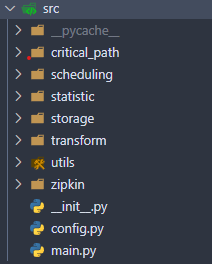
\includegraphics[width=0.35\textwidth]{resources/ch4/packages.png}
	\caption{Implementasi modul sebagai \textit{package}}
	\label{package}
\end{figure} 

%Gambar \ref{api_docs} adalah hasil tangkapan layar dokumentasi API yang disediakan oleh FastAPI. 
%\begin{figure}[!htb]
%	\centering
%	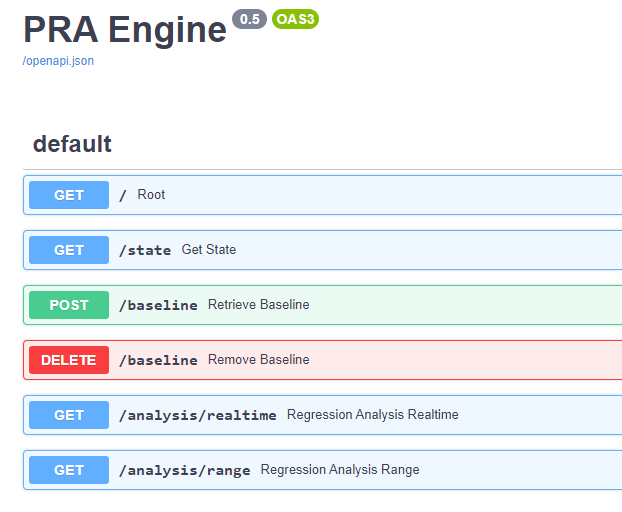
\includegraphics[width=0.5\textwidth]{resources/ch4/api_docs.png}
%	\caption{Dokumentasi API}
%	\label{api_docs}
%\end{figure} 
%
%Berikut adalah tangkapan layar dari hasil pemanggilan beberapa \textit{endpoint} yang dilakukan dengan aplikasi Postman \footnote{\url{https://www.postman.com/}}.
%\begin{figure}[h!]
%	\centering
%	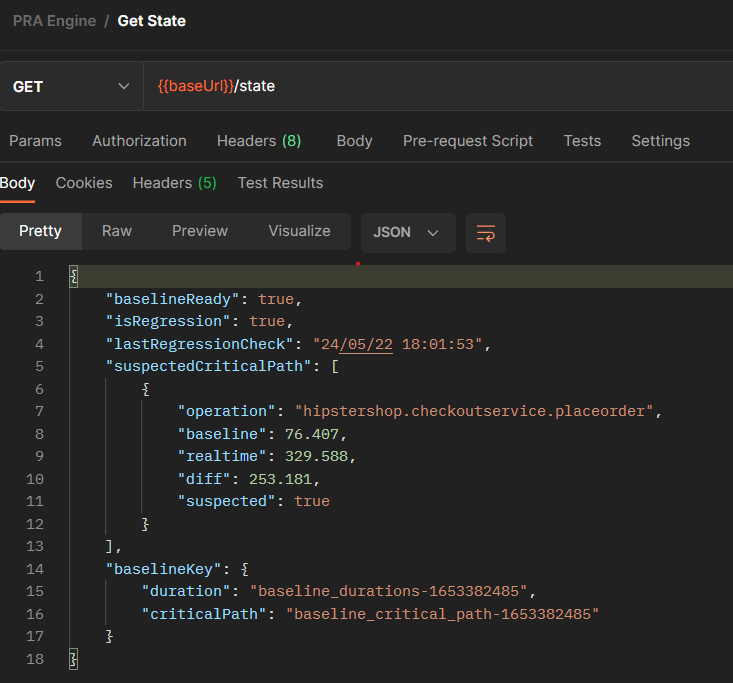
\includegraphics[width=0.75\textwidth]{resources/ch4/result_state.png}
%	\caption{Hasil pemanggilan \textit{endpoint} \texttt{/state}}
%	\label{api_state}
%\end{figure} 
%\begin{figure}[h!]
%	\centering
%	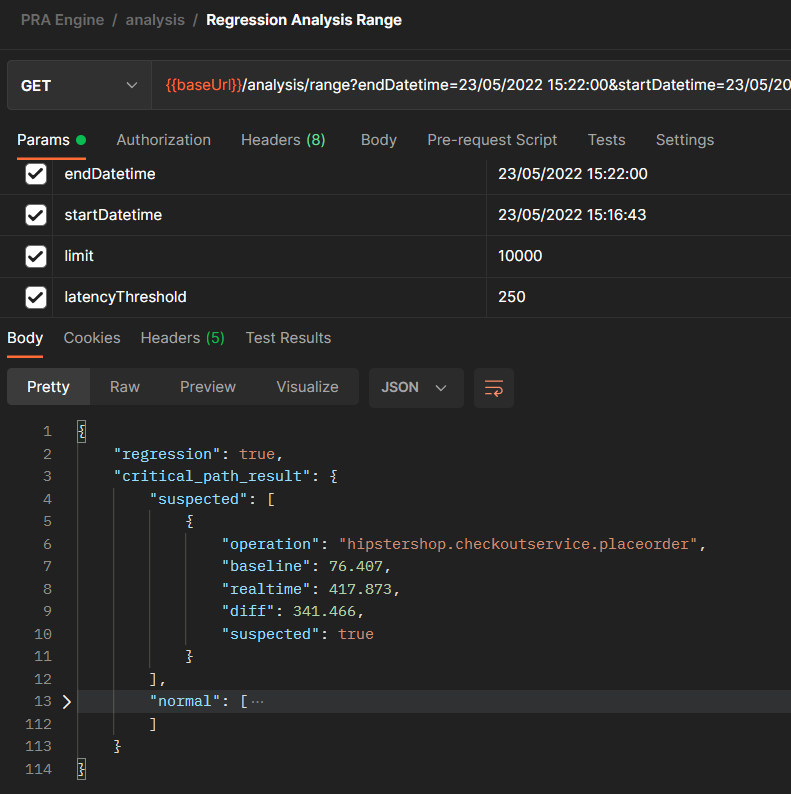
\includegraphics[width=0.75\textwidth]{resources/ch4/result_analysis_range.png}
%	\caption{Hasil pemanggilan \textit{endpoint} \texttt{/analysis/range}}
%	\label{api_analysis_range}
%\end{figure} 
%\begin{figure}[h!]
%	\centering
%	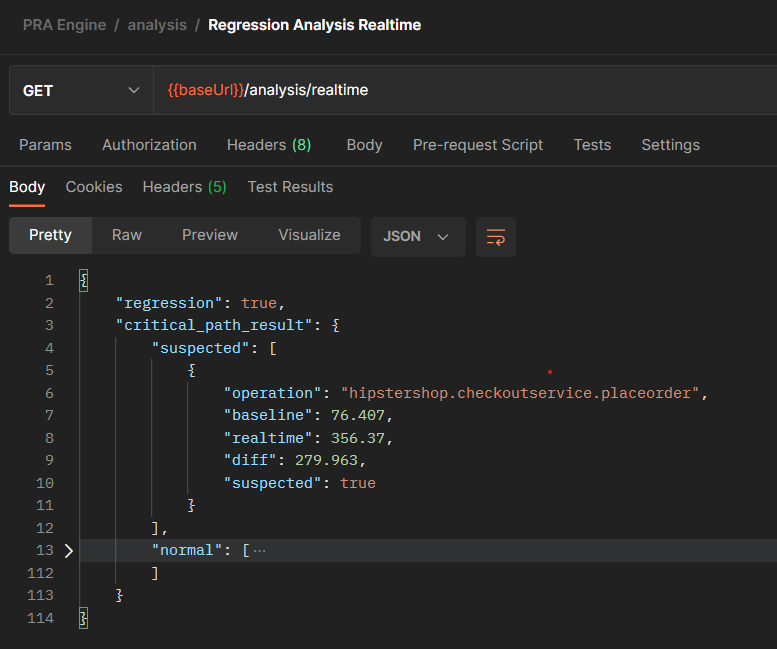
\includegraphics[width=0.75\textwidth]{resources/ch4/result_analysis_realtime.png}
%	\caption{Hasil pemanggilan \textit{endpoint} \texttt{/analysis/realtime}}
%	\label{api_analysis_realtime}
%\end{figure} 

\pagebreak


\subsubsection{Model dan Struktur Data}
Sistem PRA yang dibuat bergantung pada data \textit{trace} yang diperoleh dari Zipkin. Data tersebut tidak bisa begitu saja digunakan untuk menjalankan fungsi-fungsi dari \textit{engine} PRA sesuai yang terdapat pada gambar \ref{alur-pra} dan perlu ditransformasikan menjadi model dan struktur data yang lebih bermakna seperti yang telah disebutkan pada EM-2 di tabel \ref{engine-module}.

Dalam dokumentasinya, Zipkin menyediakan keterangan mengenai model data \textit{trace} yang digunakannya seperti yang terdapat pada \citep{zipkin-data}. Model data yang digunakan Zipkin terbagi menjadi dua yaitu \textit{span} dan \textit{trace}. \textit{Trace} sendiri merupakan serangkaian \textit{span} dengan id \textit{trace} sama yang merepresentasikan alur jalannya sebuah \textit{request} dalam sebuah \textit{service} yang telah terinstrumentasi, sementara \textit{span} merepresentasikan salah satu operasi yang terjadi sepanjang sebuah \textit{request}. Beberapa informasi yang terdapat pada data \textit{span} antara lain adalah informasi mengenai \textit{trace} dimana \textit{span} itu berada, metadata mengenai operasi yang direpresentasikan \textit{span}, durasi atau \textit{latency} dari operasi.

Sementara itu, untuk memenuhi fungsi-fungsi pada sistem PRA, data yang bersumber dari Zipkin perlu ditransformasikan menjadi struktur data yang sesuai dengan kebutuhan masing-masing tahap analisis. Dari rancangan alur sistem PRA, terdapat tiga tahap analisis yang akan dilakukan, yaitu tahap pendeteksian regresi dengan analisis statistik Kolmogorov-Smirnov, tahap analisis korelasi, dan tahap analisis \textit{critical path}.

Pada tahap pendeteksian regresi dengan tes statistik Kolmogorov-Smirnov (K-S), data yang diperlukan adalah data \textit{latency} atau durasi operasi dari \textit{span} yang dimiliki oleh Zipkin. Tes K-S akan membandingkan dua buah sampel data \textit{latency} dan akan menghasilkan hipotesis apakah kedua fungsi tersebut berada pada distribusi yang sama.

Pada tahap analisis \textit{critical path}, data yang dibutuhkan adalah pasangan \textit{key-value} dari nama operasi yang terrekam oleh Zipkin dan juga nilai \textit{latency} dari operasi tersebut. Data \textit{critical path} akan disimpan sebagai struktur data \textit{map} yang sesuai untuk menyimpan data berbentuk pasangan \textit{key-value}. Data ini akan didapatkan dari data \textit{trace} bawaan Zipkin yang sudah memiliki informasi mengenai \textit{critical path} dan juga nilai \textit{latency} nya masing-masing. 

\subsubsection{Algoritma}
Setelah pada subbab sebelumnya didefinisikan struktur data yang akan digunakan untuk merepresentasikan beberapa model seperti yang ada pada gambar \ref{alur-pra}, pada subbab ini akan didefinisikan algoritma penting yang akan digunakan untuk melakukan pendeteksian regresi pada aplikasi Microservice. 

algoritma yang didasarkan pada tes statistik Kolmogorov-Smirnov ini akan membandingkan dua buah sampel data dan akan menentukan apakah kedua sampel tersebut berasal dari distribusi yang sama. Pertama-tama kita definisikan dua hipotesis yaitu $h_{0}$ atau hipotesis \textit{null} yang menyatakan bahwa kedua sampel data berasal dari distribusi yang sama dan $h_{a}$ atau hipotesis alternatif yang menyatakan bahwa kedua sampel data berasal dari dua distribusi yang berbeda. 

Kemudian akan dijalankan tes statistik K-S yang dilakukan menggunakan fungsi dari \textit{library}
SciPy yang akan menghasilkan dua buah nilai, yaitu \texttt{statistic} dan \texttt{p-value}. Jika nilai \texttt{p-value} lebih kecil dari nilai signifikan, atau \texttt{alpha} pada fungsi,  maka kita dapat menolak $h_{0}$ dan menerima $h_{a}$. Jika  \texttt{p-value} tidak lebih kecil dari nilai signifikan, maka selanjutnya adalah membandingkan antara nilai \texttt{statistic} dan \texttt{critical value}. \texttt{Critical value} sendiri merupakan sebuah titik pada tes hipotesis yang akan dibandingkan pada hasil nilai \texttt{statistic} yang akan digunakan untuk menolak atau menerima hipotesis \textit{null}. Jika nilai \texttt{statistic} lebih besar dari nilai \texttt{critical value}, maka kita dapat menolak $h_{0}$ dan menerima $h_{a}$ atau artinya kedua sampel data berasal dari distribusi yang berbeda. Namun jika  nilai \texttt{statistic} lebih kecil dari nilai \texttt{critical value}, kita tidak dapat menolak $h_{0}$ atau artinya kedua sampel data berasal dari distribusi yang sama.


Jika kedua sampel ternyata berasal dari distribusi yang berbeda, maka dapat dicurigai telah terjadi regresi pada aplikasi sebab distribusi dari data yang bersumber dari  \textit{trace} periodikal berbeda dengan distribusi dari data \textit{trace} \textit{baseline} yang dijadikan acuan kinerja normal aplikasi.

\lstinputlisting[captionpos=b, language=Python,caption={Algoritma tes statistik Kolmogorov-Smirnov}]{codes/ch4/ks.py}


\subsection{Implementasi PRA UI}
Komponen lainnya yang akan diimplementasikan pada Tugas Akhir ini adalah komponen \textit{User Interface} (UI). Komponen ini akan menjadi antarmuka yang dapat digunakan untuk mengetahui \textit{state} dari sistem PRA. Fungsionalitas yang akan dibuat pada komponen UI akan dijabarkan pada tabel kebutuhan  fungsional \ref{ui-functional}.
\begin{small}
	\begin{longtable}{ | p{3cm} | p{9cm} | }
		\caption{Tabel kebutuhan fungsional komponen UI}
		\label{ui-functional}                                                           
		\\ \hline
		\centering\bfseries{ID} & \centering\bfseries{Deskripsi} \tabularnewline \hline
		\endfirsthead
		\centering{UI-1} & UI dapat menampilkan status pendeteksian regresi  \\ \hline
		\centering{UI-2} & UI dapat menampilkan hasil analisis \textit{critical path} berupa nama operasi dan nilai \textit{latency} \\ \hline

	\end{longtable}
\end{small}

\subsubsection{Hasil implementasi}
Berikut adalah tangkapan layar hasil implementasi komponen PRA UI.

\begin{figure}[!htb]
	\centering
	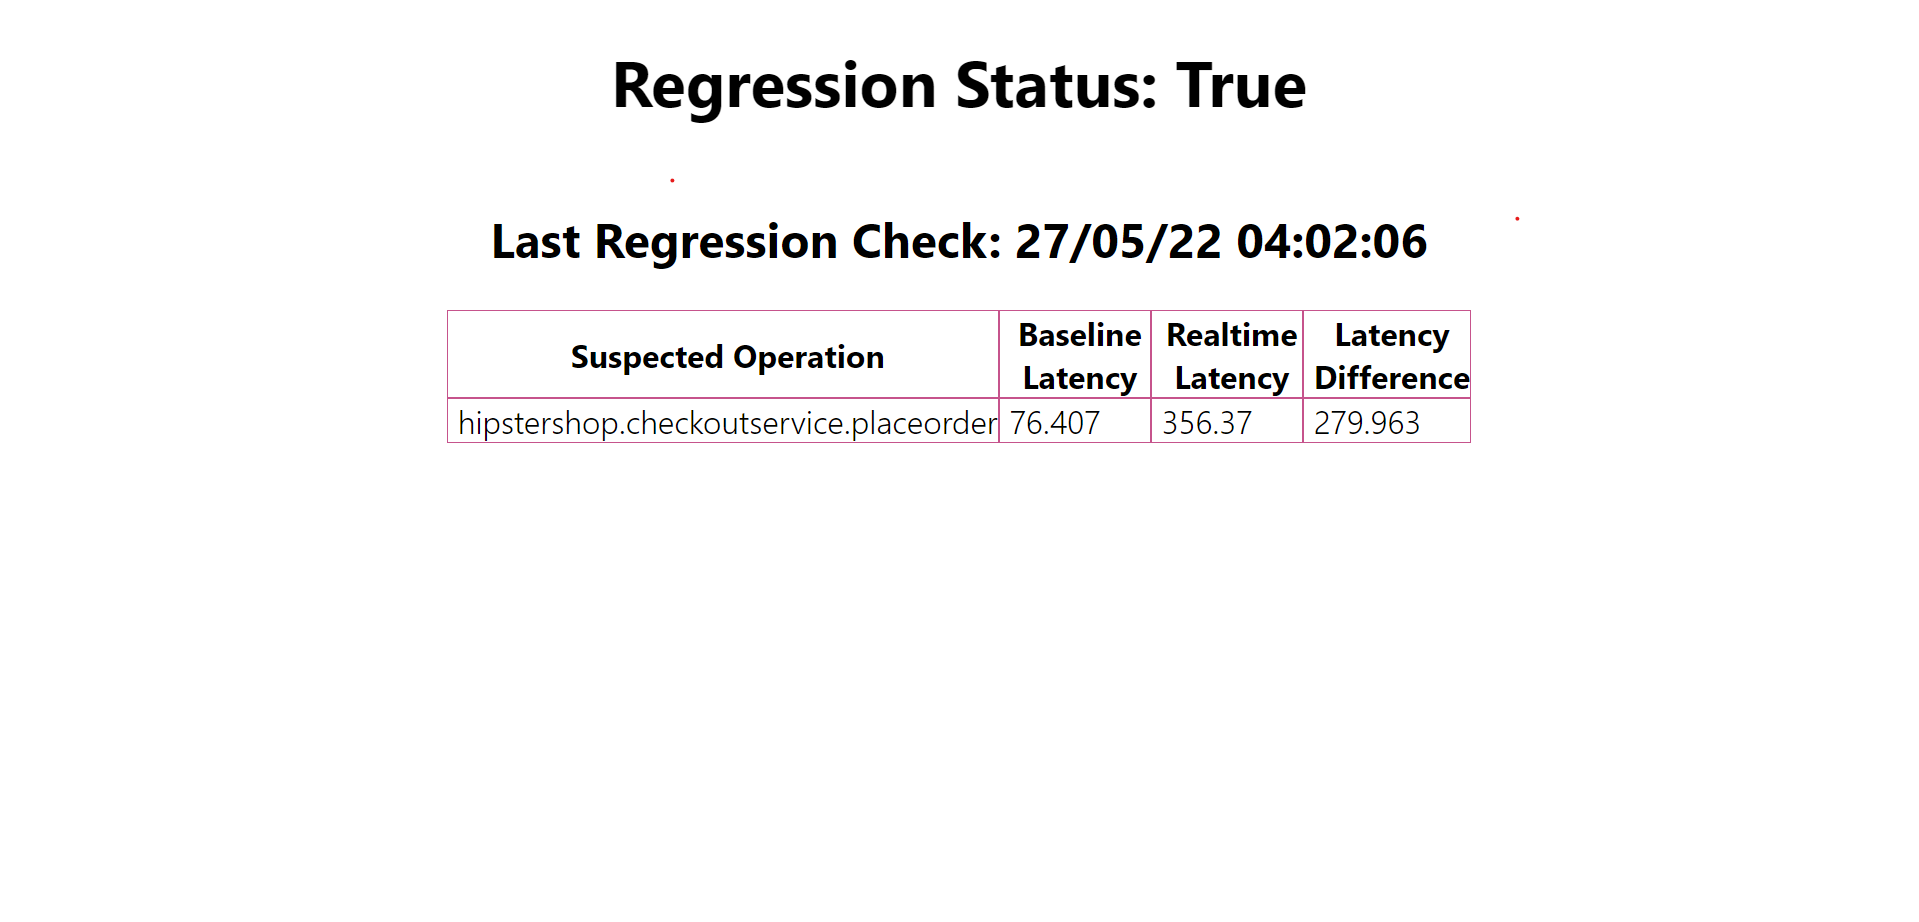
\includegraphics[width=1\textwidth]{resources/ch4/ui.png}
	\caption{Tangkapan layar UI}
	\label{ui}
\end{figure}

\section{Pengujian}
Untuk mengetahui keberhasilan dari sistem yang telah diimplementasikan, akan dilakukan pengujian sebagai berikut.
\subsection{Tujuan Pengujian}
Pengujian sistem PRA akan dilakukan dengan tujuan untuk:
\begin{enumerate}
	\item Mengukur keberhasilan sistem PRA dalam mendeteksi regresi
	\item Mengukur keberhasilan sistem PRA dalam menentukan kandidat sumber regresi
	\item Mengukur \textit{overhead} yang diakibatkan oleh sistem PRA dengan
	indikator berupa penggunaan memori dan pemanfaatan CPU.
\end{enumerate}

Tujuan utama pengujian sistem \textit{Performance Regression Analysis} adalah untuk menguji apakah sistem dapat mendeteksi terjadinya regresi atau penurunan kinerja dengan indikasi peningkatan nilai \textit{latency} yang disebabkan oleh perubahan yang terjadi pada aplikasi. Perubahan tersebut dapat berupa penambahan atau \textit{update} fitur, hasil perbaikan \textit{bug}, dsb. Sehingga kasus-kasus yang akan diujikan utamanya merupakan simulasi terjadinya perubahan pada level aplikasi \textit{microservice}. Namun sebagai perbandingan akan terdapat juga kasus-kasus yang menyimulasikan perubahan yang terjadi di luar level aplikasi seperti peningkatan jumlah pengguna dan peningkatan \textit{load} pada Load Generator pada \textit{service}-\textit{service} tertentu. Kasus pengujian akan dijelaskan lebih lanjut pada subbab \ref{metode-pengujian}.

\subsection{Lingkungan Pengujian}
Pengujian akan dilakukan pada Google Kubernetes Engine dengan spesifikasi yang dipaparkan pada tabel \ref{testing-env}.
\begin{small}
	\begin{longtable}{ | p{5cm} | p{8cm} | }
		\caption{Spesifikasi Lingkungan Pengujian}
		\label{testing-env}                                                           
		\\ \hline
		\centering\bfseries{Layanan Kubernetes} & \centering\bfseries{Google Kubernetes Engine} \tabularnewline \hline
		\endfirsthead
		\textit{Operating System} & Container Optimized OS (COS) \\ \hline
		\textit{Instance Type} & n1-standard-2 (2 vCPU,  7,5 GiB RAM) \\ \hline
		Jumlah Node & 3 \\ \hline
		
	\end{longtable}
\end{small}

\subsection{Aplikasi Pengujian}
Aplikasi yang akan digunakan untuk melakukan pengujian sistem PRA adalah aplikasi Hipster Shop yang merupakan aplikasi \textit{e-commerce} berbasis web yang dibuat untuk mendemostrasikan berbagai macam teknologi yang dimiliki oleh Google. Seperti pada gambar \ref{butiq-arch}, Hipster Shop terdiri atas 10 microservice yang saling berkomunikasi melalui gRPC. Selain itu Hipster Shop juga memiliki load generator yang secara terus menerus mengirimkan request untuk menyimulasikan alur belanja pengguna. Hipster Shop sudah memiliki load generator yang dibuat menggunakan Locust
untuk menyimulasikan pengunaan aplikasi oleh sejumlah user. Aplikasi Hipster Shop akan dimodifikasi dengan diinstumentasikan menggunakan Zipkin untuk menyimulasikan lingkungan \textit{distributed tracing} yang menggunakan Zipkin.
\begin{figure}[!htb]
	\centering
	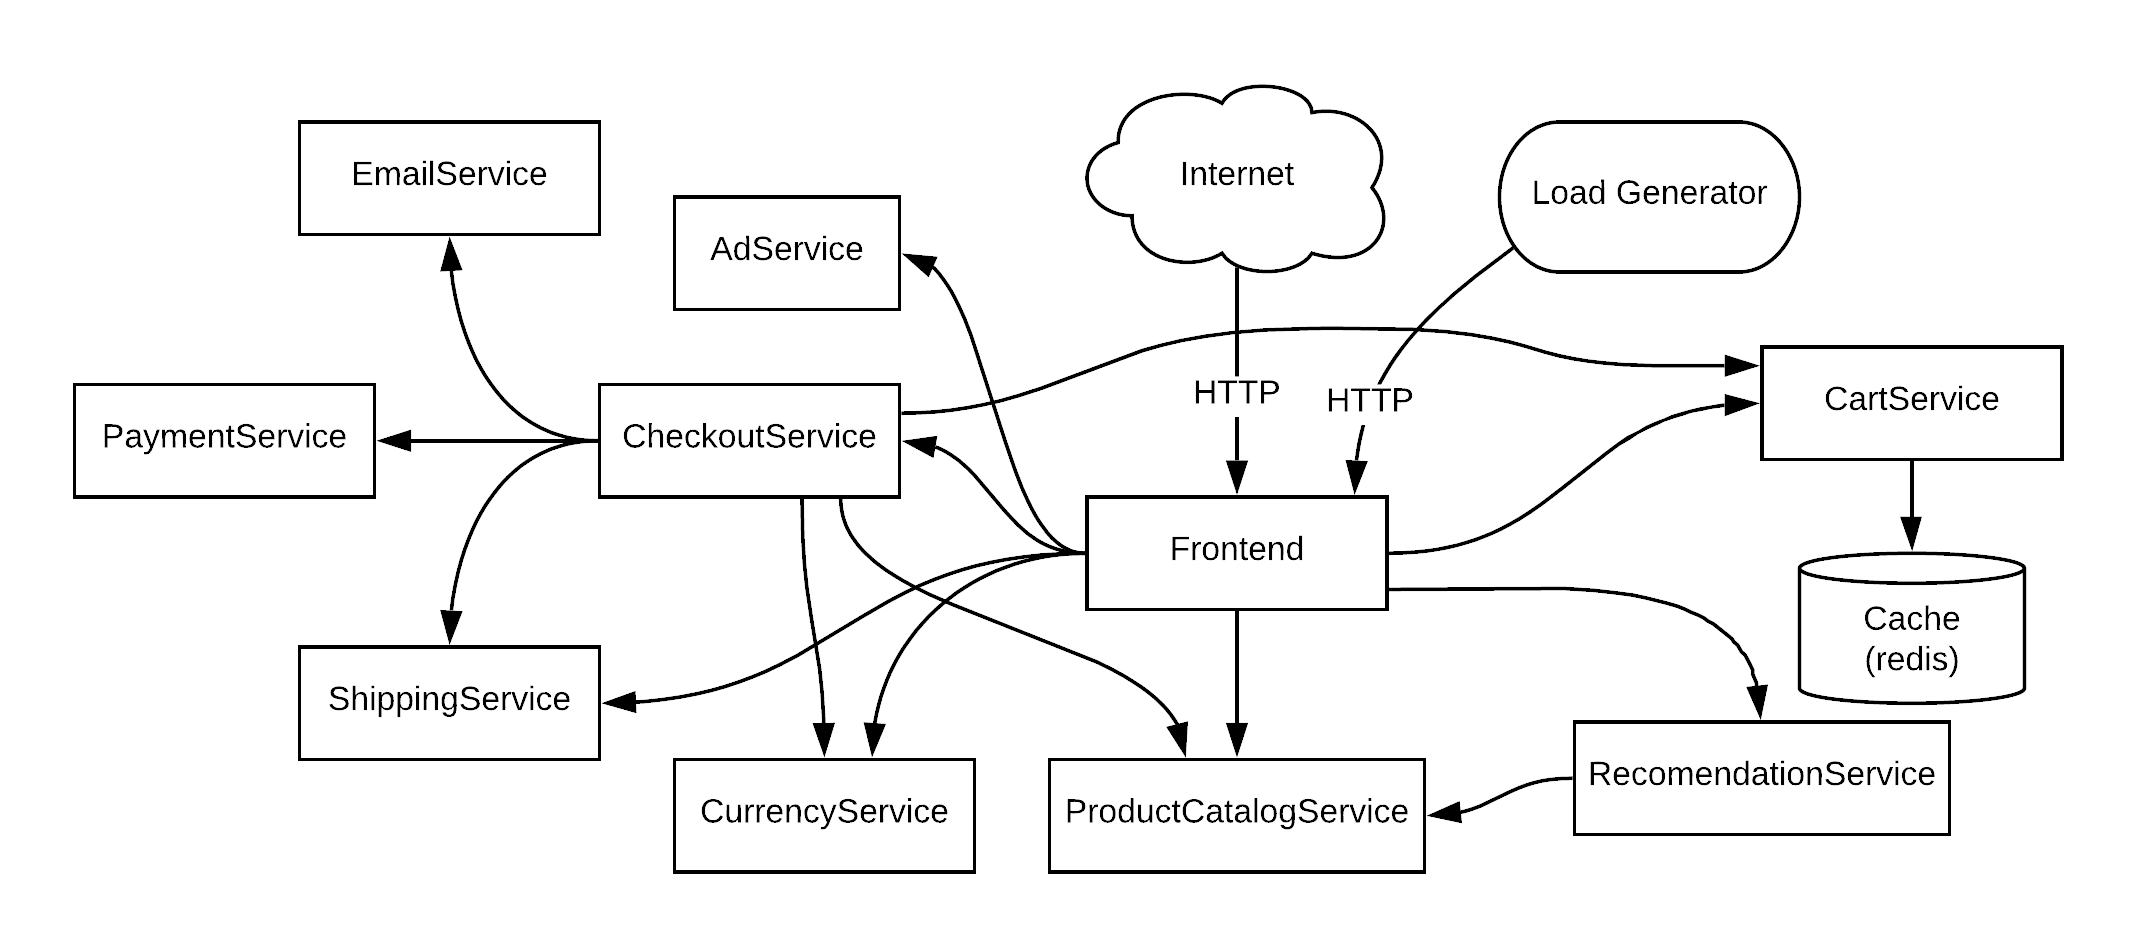
\includegraphics[width=1\textwidth]{resources/ch4/hipster-arch.png}
	\caption{Arsitektur aplikasi Hipster Shop}
	\label{butiq-arch}
\end{figure}

\pagebreak


\subsection{Metode Pengujian}
\label{metode-pengujian}
Untuk melakukan pengujian pada sistem PRA yang telah dibuat, \textit{service} yang ada pada Hipster Shop akan dimodifikasi untuk meniru perilaku dari \textit{service} yang mengalami regresi kinerja. Ada dua metode utama yang dapat dilakukan untuk membuat perilaku regresi pada \textit{service} yaitu dengan menambahkan perintah \textit{sleep} dan menambahkan \textit{loop} dengan operasi \textit{dereference} sebuah variabel yang membutuhkan banyak usaha dari CPU untuk menyelesaikannya sehingga diharapkan fungsi-fungsi tersebut akan memiliki \textit{latency} yang lebih besar. 

Ada dua tahap yang akan dilakukan untuk melakukan pengujian ini, pertama tahap pengambilan data \textit{baseline}. Data \textit{baseline} akan diambil dengan menyimulasikan pengunaan aplikasi dengan menggunakan Load Generator yang akan dijalankan dengan variabel \textbf{25 User} dan \textbf{5 Spawn Rate} selama \textbf{1 jam}. Data \textit{baseline} ini kemudian akan disimpan oleh \textit{engine} untuk dipergunakan di kasus-kasus pengujian selanjutnya. Tahap selanjutnya adalah melakukan pengujian dengan kasus-kasus yang akan dijelaskan lebih lanjut.

Terdapat dua jenis kasus uji yang akan diujikan pada sistem. Jenis pertama adalah kasus-kasus yang menyimulasikan regresi dengan melakukan perubahan yang terjadi di level aplikasi dengan cara melakukan modifikasi secara sengaja di level kode. Kasus pertama akan memiliki ID dengan awalan \textbf{SI} menandakan \textit{skenario-internal}. Jenis kedua adalah kasus-kasus yang menyimulasikan regresi dengan meningkatkan jumlah pengguna dan \textit{load} pada Load Generator. Kasus kedua akan memliki ID dengan awalan \textbf{SE} menandakan \textit{skenario-eksternal}. Tabel \ref{testcase} akan menjelaskan kasus-kasus pengujian sistem.

Pengujian pada tabel \ref{testcase} seluruhnya dilakukan dengan cara terlebih dahulu melakukan \textit{deployment} masing-masing kasus uji di lingkungan Kubernetes kemudian menjalankan aplikasi Load Generator sesuai dengan spesifikasi masing-masing kasus uji selama $\pm 5$ menit. Pengujian akan dilakukan dengan memanggil \textit{endpoint} \texttt{/analysis/range} dengan parameter StartTime dan EndTime yang sesuai dengan kasus uji. 

Untuk keperluan pengujian akan digunakan 3 level signifikan atau alpha yang berbeda yaitu 0,1, 0,05, dan 0,001. Ketiga level signifikan ini digunakan untuk mengetahui sensitivitas hasil pendeteksian regresi dengan arti semakin kecil nilai signifikan, maka akan semakin signifikan bukti untuk menolak $h_{0}$. Nilai signifikan 0,1 dipilih sebagai batas atas nilai signifikan untuk mengetahui tingkat sensitivitas dari kasus uji dengan nilai signifikan yang paling besar. Sementara nilai 0,05 dipilih sebab nilai tersebut merupakan nilai yang paling umum digunakan sebagai nilai signifikan pada tes statistik hipotesis. Sementara nilai 0,001 dipilih sebagai perbandingan nilai signifikan paling kecil untuk menguji batas bawah dari nilai signifikan.

Hasil akhir dari setiap kasus uji akan berupa \textit{response} dalam bentuk JSON dari API dan juga \textit{log} dari aplikasi untuk mengetahui hasil tes  statistik K-S yang akan dipergunakan untuk keperluan analisis selanjutnya.
\begin{table}[htb]
	\caption{Tabel kasus uji}
	
	\begin{adjustwidth}{-1.5cm}{}
		% Please add the following required packages to your document preamble:
		% \usepackage{multirow}
		% \usepackage[table,xcdraw]{xcolor}
		% If you use beamer only pass "xcolor=table" option, i.e. \documentclass[xcolor=table]{beamer}
		\begin{tabular}{llccl}
			\hline
			\rowcolor[HTML]{009901} 
			\multicolumn{1}{c}{\cellcolor[HTML]{009901}{\color[HTML]{FFFFFF} \textbf{ID}}} &
			\multicolumn{1}{c}{\cellcolor[HTML]{009901}{\color[HTML]{FFFFFF} \textbf{Service (Fungsi)}}} &
			\multicolumn{1}{l}{\cellcolor[HTML]{009901}{\color[HTML]{FFFFFF} \textbf{Extra Latency}}} &
			\multicolumn{1}{l}{\cellcolor[HTML]{009901}{\color[HTML]{FFFFFF} \textbf{User}}} &
			{\color[HTML]{FFFFFF} \textbf{Keterangan}} \\ \hline
			\multicolumn{1}{|l|}{\textbf{SI1}} &
			\multicolumn{1}{l|}{CheckoutService (placeorder)} &
			\multicolumn{1}{c|}{100ms} &
			\multicolumn{1}{c|}{25} &
			\multicolumn{1}{l|}{Kasus extra latency \#1} \\ \hline
			\multicolumn{1}{|l|}{\textbf{SI2}} &
			\multicolumn{1}{l|}{CheckoutService (placeorder)} &
			\multicolumn{1}{c|}{250ms} &
			\multicolumn{1}{c|}{25} &
			\multicolumn{1}{l|}{Kasus extra latency \#2} \\ \hline
			\multicolumn{1}{|l|}{\textbf{SI3}} &
			\multicolumn{1}{l|}{CheckoutService (placeorder)} &
			\multicolumn{1}{c|}{350ms} &
			\multicolumn{1}{c|}{25} &
			\multicolumn{1}{l|}{Kasus extra latency \#3} \\ \hline
			\multicolumn{1}{|l|}{\textbf{SI4}} &
			\multicolumn{1}{l|}{CheckoutService (placeorder)} &
			\multicolumn{1}{c|}{250ms} &
			\multicolumn{1}{c|}{75} &
			\multicolumn{1}{l|}{\begin{tabular}[c]{@{}l@{}}Kasus extra latency \\ dengan peningkatan user \#1\end{tabular}} \\ \hline
			\multicolumn{1}{|l|}{\textbf{SI5}} &
			\multicolumn{1}{l|}{CheckoutService (placeorder)} &
			\multicolumn{1}{c|}{250ms} &
			\multicolumn{1}{c|}{150} &
			\multicolumn{1}{l|}{\begin{tabular}[c]{@{}l@{}}Kasus extra latency \\ dengan peningkatan user \#1\end{tabular}} \\ \hline
			\multicolumn{1}{|l|}{\textbf{SI6}} &
			\multicolumn{1}{l|}{CheckoutService (placeorder)} &
			\multicolumn{1}{c|}{-} &
			\multicolumn{1}{c|}{25} &
			\multicolumn{1}{l|}{Kasus peningkatan kerja CPU} \\ \hline
			\multicolumn{1}{|l|}{} &
			\multicolumn{1}{l|}{CheckoutService (placeorder)} &
			\multicolumn{1}{c|}{} &
			\multicolumn{1}{c|}{} &
			\multicolumn{1}{l|}{} \\ \cline{2-2}
			\multicolumn{1}{|l|}{} &
			\multicolumn{1}{l|}{\begin{tabular}[c]{@{}l@{}}ProductCatalog (getproduct,\\ listproducts)\end{tabular}} &
			\multicolumn{1}{c|}{} &
			\multicolumn{1}{c|}{} &
			\multicolumn{1}{l|}{} \\ \cline{2-2}
			\multicolumn{1}{|l|}{} &
			\multicolumn{1}{l|}{ShippingService (getquote)} &
			\multicolumn{1}{c|}{} &
			\multicolumn{1}{c|}{} &
			\multicolumn{1}{l|}{} \\ \cline{2-2}
			\multicolumn{1}{|l|}{\multirow{-4}{*}{\textbf{SI7}}} &
			\multicolumn{1}{l|}{\begin{tabular}[c]{@{}l@{}}RecommendationService \\ (listrecommendations)\end{tabular}} &
			\multicolumn{1}{c|}{\multirow{-4}{*}{250ms}} &
			\multicolumn{1}{c|}{\multirow{-4}{*}{25}} &
			\multicolumn{1}{l|}{\multirow{-4}{*}{\begin{tabular}[c]{@{}l@{}}Kasus extra latency\\  dengan beberapa service\end{tabular}}} \\ \hline
			\multicolumn{1}{|l|}{\textbf{SE1}} &
			\multicolumn{1}{l|}{All Normal} &
			\multicolumn{1}{c|}{-} &
			\multicolumn{1}{c|}{75} &
			\multicolumn{1}{l|}{\begin{tabular}[c]{@{}l@{}}Tidak ada peningkatan latency\\ dengan peningkatan pengguna \#1\end{tabular}} \\ \hline
			\multicolumn{1}{|l|}{\textbf{SE2}} &
			\multicolumn{1}{l|}{All Normal} &
			\multicolumn{1}{c|}{-} &
			\multicolumn{1}{c|}{150} &
			\multicolumn{1}{l|}{\begin{tabular}[c]{@{}l@{}}Tidak ada peningkatan latency\\ dengan peningkatan pengguna \#1\end{tabular}} \\ \hline
			\multicolumn{1}{|l|}{\textbf{SE3}} &
			\multicolumn{1}{l|}{\begin{tabular}[c]{@{}l@{}}Checkout load \\ increased to 100 in loadgen\end{tabular}} &
			\multicolumn{1}{c|}{-} &
			\multicolumn{1}{c|}{25} &
			\multicolumn{1}{l|}{Tes pengujian load external \#1} \\ \hline
			\multicolumn{1}{|l|}{\textbf{SE4}} &
			\multicolumn{1}{l|}{\begin{tabular}[c]{@{}l@{}}Currency load\\  increased to 100 in loadgen\end{tabular}} &
			\multicolumn{1}{c|}{-} &
			\multicolumn{1}{c|}{25} &
			\multicolumn{1}{l|}{Tes pengujian load external \#2} \\ \hline
		\end{tabular}
	\end{adjustwidth}
	\label{testcase}
\end{table}
\pagebreak

\subsection{Hasil Pengujian Regresi}
Berikut adalah hasil pengujian yang telah dilakukan pada sistem PRA sesuai dengan kasus uji seperti yang telah dijabarkan pada tabel \ref{testcase}. Hasil tangkapan layar dari aplikasi Postman terdapat pada lampiran \ref{lampiran_a}.

\subsubsection{Kasus SI1}
Pada kasus ini di semua nilai alpha, regresi terdeteksi pada nilai alpha 0.1 namun tidak terdeteksi pada nilai alpha 0.05 dan 0.001. Analisis \textit{critical path} dapat menentukan sumber regresi pada nilai alpha 0.1 yaitu operasi \texttt{placeorder} dari \textit{service} \texttt{CheckoutService} dengan selisih perbedaan \textit{latency} sebesar 126ms.

\subsubsection{Kasus SI2}
Pada kasus ini di semua nilai alpha, regresi terdeteksi dan analisis \textit{critical path} dapat menentukan sumber regresi yaitu operasi \texttt{placeorder} dari \textit{service} \texttt{CheckoutService} dengan selisih perbedaan \textit{latency} sebesar 268ms. Analisis \textit{critical path} sudah dapat dengan benar menentukan sumber regresi sesuai dengan kasus uji.

\subsubsection{Kasus SI3}
Pada kasus ini di semua nilai alpha, regresi terdeteksi dan analisis \textit{critical path} dapat menentukan sumber regresi yaitu operasi \texttt{placeorder} dari \textit{service} \texttt{CheckoutService} dengan selisih \textit{latency} sebesar 338ms. Analisis \textit{critical path} sudah dapat dengan benar menentukan sumber regresi sesuai dengan kasus uji.

\subsubsection{Kasus SI4}
Pada kasus ini di semua nilai alpha, regresi terdeteksi dan analisis \textit{critical path} dapat menentukan sumber regresi yaitu operasi \texttt{placeorder} dari \textit{service} \texttt{CheckoutService} dengan selisih \textit{latency} sebesar 282ms. Analisis \textit{critical path} sudah dapat dengan benar menentukan sumber regresi sesuai dengan kasus uji.

\subsubsection{Kasus SI5}
Pada kasus ini di semua nilai alpha, regresi terdeteksi dan analisis \textit{critical path} dapat menentukan sumber regresi yaitu operasi \texttt{placeorder} dari \textit{service} \texttt{CheckoutService} dengan selisih \textit{latency sebesar} 314ms. Analisis \textit{critical path} sudah dapat dengan benar menentukan sumber regresi sesuai dengan kasus uji.


\subsubsection{Kasus SI6}
Pada kasus ini, regresi terdeteksi dan analisis \textit{critical path} dapat menentukan sumber regresi yaitu operasi \texttt{placeorder} dari \textit{service} \texttt{CheckoutService} dengan selisih \textit{latency} sebesar 201ms. Analisis \textit{critical path} sudah dapat dengan benar menentukan sumber regresi sesuai dengan kasus uji.


\subsubsection{Kasus SI7}
Pada kasus ini di semua nilai alpha, regresi terdeteksi dan analisis \textit{critical path} dapat menentukan sumber regresi yaitu operasi \texttt{placeorder} dari \textit{service} \texttt{Checkout Service}, operasi \texttt{listrecommendations} dari \textit{service} \texttt{Recommendation Service}, operasi \texttt{getproduct} dari \textit{service} \texttt{ProductCatalog Service}, \texttt{listproducts} dari \textit{service} \texttt{ProductCatalog Service}, dan operasi \texttt{getquote} dari \textit{service} \texttt{Shipping Service}. Analisis \textit{critical path} sudah dapat dengan benar menentukan sumber regresi sesuai dengan kasus uji.


\subsubsection{Kasus SE1}
Pada kasus ini di semua nilai alpha, regresi terdeteksi namun analisis \textit{critical path} tidak dapat menentukan sumber regresi sebab selisih \textit{latency} tidak cukup besar sehingga tidak terdeteksi di data \textit{suspected}, namun dari data normal terlihat bahwa operasi-operasi hanya memiliki selisih \textit{latency} dari 0ms sampai dengan 4ms sehingga penyebab regresi bukanlah salah satu operasi di sebuah \textit{service} melainkan karena faktor eksternal, oleh karena itu walaupun analisis \textit{critical path} tidak dapat menentukan sumber regresi, hasilnya sudah tepat sebab penyebab regresi merupakan faktor eksternal bukan faktor internal.

\subsubsection{Kasus SE2}
Pada kasus ini di semua nilai alpha, regresi terdeteksi namun analisis \textit{critical path} tidak dapat menentukan sumber regresi sebab selisih \textit{latency} tidak cukup besar sehingga tidak terdeteksi di data \textit{suspected}, namun dari data normal terlihat bahwa operasi-operasi hanya memiliki selisih \textit{latency} dari 12ms sampai dengan 34ms sehingga penyebab regresi bukanlah salah satu operasi di sebuah \textit{service} melainkan karena faktor eksternal, oleh karena itu walaupun analisis \textit{critical path} tidak dapat menentukan sumber regresi, hasilnya sudah tepat sebab penyebab regresi merupakan faktor eksternal bukan faktor internal.

\subsubsection{Kasus SE3}
Pada kasus ini di semua nilai alpha, regresi terdeteksi namun analisis \textit{critical path} tidak dapat menentukan sumber regresi sebab selisih \textit{latency} tidak cukup besar sehingga tidak terdeteksi di data \textit{suspected}, namun dari data normal terlihat bahwa operasi-operasi hanya memiliki selisih \textit{latency} dari 3ms sampai dengan 28ms sehingga penyebab regresi bukanlah salah satu operasi di sebuah \textit{service} melainkan karena faktor eksternal, oleh karena itu walaupun analisis \textit{critical path} tidak dapat menentukan sumber regresi, hasilnya sudah tepat sebab penyebab regresi merupakan faktor eksternal bukan faktor internal.
 
\subsubsection{Kasus SE4}
Pada kasus ini di semua nilai alpha, regresi terdeteksi namun analisis \textit{critical path} tidak dapat menentukan sumber regresi sebab selisih \textit{latency} tidak cukup besar sehingga tidak terdeteksi di data \textit{suspected}, namun dari data normal terlihat bahwa operasi-operasi hanya memiliki selisih \textit{latency} dari 1ms sampai dengan 2ms sehingga penyebab regresi bukanlah salah satu operasi di sebuah \textit{service} melainkan karena faktor eksternal, oleh karena itu walaupun analisis \textit{critical path} tidak dapat menentukan sumber regresi, hasilnya sudah tepat sebab penyebab regresi merupakan faktor eksternal bukan faktor internal.

\subsubsection{Ringkasan hasil pengujian}
Tabel-tabel berikut mendeskripsikan ringkasan hasil pengujian yang telah dilakukan dengan ketiga nilai alpha yang berbeda-beda. Hasilnya adalah pada semua kasus pengujian, kasus SI2 sampai dengan kasus SE4 berhasil dideteksi regresi dan analisis \textit{critical path}-nya sesuai. Hanya saja untuk kasus SI1, hanya nilai alpha 0,1 yang dapat berhasil mendeteksi regresi dan menentukan sumber penyebab regresi dengan analisis \textit{critical path}. Nilai alpha lain tidak dapat mendeteksi regresi dan tidak melakukan analisis \textit{critical path}.

\begin{table}[!htb]
	\caption{Ringkasan hasil pengujian dengan alpha 0,1}
	\centering
	\begin{tabular}{|l|c|c|}
		\hline
		\rowcolor[HTML]{3166FF} 
		{\color[HTML]{FFFFFF} ID} &
		\multicolumn{1}{l|}{\cellcolor[HTML]{3166FF}{\color[HTML]{FFFFFF} Regresi terdeteksi}} &
		\multicolumn{1}{l|}{\cellcolor[HTML]{3166FF}{\color[HTML]{FFFFFF} Hasil Critical Path sesuai}} \\ \hline
		\textbf{SI1} & Ya & Ya \\ \hline
		\textbf{SI2} & Ya    & Ya    \\ \hline
		\textbf{SI3} & Ya    & Ya    \\ \hline
		\textbf{SI4} & Ya    & Ya    \\ \hline
		\textbf{SI5} & Ya    & Ya    \\ \hline
		\textbf{SI6} & Ya    & Ya    \\ \hline
		\textbf{SI7} & Ya    & Ya    \\ \hline
		\textbf{SE1} & Ya    & Ya \\ \hline
		\textbf{SE2} & Ya    & Ya \\ \hline
		\textbf{SE3} & Ya    & Ya \\ \hline
		\textbf{SE4} & Ya    & Ya \\ \hline
	\end{tabular}
	\label{test-summary-1}
\end{table}

\begin{table}[!htb]
	\caption{Ringkasan hasil pengujian dengan alpha 0,05}
	\centering
	\begin{tabular}{|l|c|c|}
		\hline
		\rowcolor[HTML]{3166FF} 
		{\color[HTML]{FFFFFF} ID} &
		\multicolumn{1}{l|}{\cellcolor[HTML]{3166FF}{\color[HTML]{FFFFFF} Regresi terdeteksi}} &
		\multicolumn{1}{l|}{\cellcolor[HTML]{3166FF}{\color[HTML]{FFFFFF} Hasil Critical Path sesuai}} \\ \hline
		\textbf{SI1} & Tidak & Tidak \\ \hline
		\textbf{SI2} & Ya    & Ya    \\ \hline
		\textbf{SI3} & Ya    & Ya    \\ \hline
		\textbf{SI4} & Ya    & Ya    \\ \hline
		\textbf{SI5} & Ya    & Ya    \\ \hline
		\textbf{SI6} & Ya    & Ya    \\ \hline
		\textbf{SI7} & Ya    & Ya    \\ \hline
		\textbf{SE1} & Ya    & Ya \\ \hline
		\textbf{SE2} & Ya    & Ya \\ \hline
		\textbf{SE3} & Ya    & Ya \\ \hline
		\textbf{SE4} & Ya    & Ya \\ \hline
	\end{tabular}
	\label{test-summary-2}
\end{table}

\begin{table}[!htb]
	\caption{Ringkasan hasil pengujian dengan alpha 0,001}
	\centering
	\begin{tabular}{|l|c|c|}
		\hline
		\rowcolor[HTML]{3166FF} 
		{\color[HTML]{FFFFFF} ID} &
		\multicolumn{1}{l|}{\cellcolor[HTML]{3166FF}{\color[HTML]{FFFFFF} Regresi terdeteksi}} &
		\multicolumn{1}{l|}{\cellcolor[HTML]{3166FF}{\color[HTML]{FFFFFF} Hasil Critical Path sesuai}} \\ \hline
		\textbf{SI1} & Tidak & Tidak \\ \hline
		\textbf{SI2} & Ya    & Ya    \\ \hline
		\textbf{SI3} & Ya    & Ya    \\ \hline
		\textbf{SI4} & Ya    & Ya    \\ \hline
		\textbf{SI5} & Ya    & Ya    \\ \hline
		\textbf{SI6} & Ya    & Ya    \\ \hline
		\textbf{SI7} & Ya    & Ya    \\ \hline
		\textbf{SE1} & Ya    & Ya \\ \hline
		\textbf{SE2} & Ya    & Ya \\ \hline
		\textbf{SE3} & Ya    & Ya \\ \hline
		\textbf{SE4} & Ya    & Ya \\ \hline
	\end{tabular}
	\label{test-summary-3}
\end{table}

\pagebreak

\subsection{Hasil Pengujian Kinerja} 
Dari 11 kasus pengujian, rata-rata kakas PRA Engine menggunakan 0,046 vCPU dengan standard deviasi 0,0038 dan 154,41 MiB Memory dengan standard deviasi 17,91 dalam sekali melakukan analisis. Keseluruhan \textit{cluster} memiliki \textit{resource} sebanyak 6 vCPU dan 22,5 GiB, sehingga dalam sekali melakukan analisis PRA Engine mengakibatkan \textit{overhead} CPU sebanyak 0,78 \% dan Memory sebanyak 0,67 \% kepada \textit{cluster} Kubernetes. \textit{Overhead} yang diakibatkan oleh kakas termasuk rendah sehingga penggunaan kakas PRA Engine tidak akan berdampak pada kinerja \textit{cluster} Kubernetes secara keseluruhan. Detail hasil pengujian kinerja terdapat pada lampiran \ref{lampiran_b}.
                           
%\subsubsection{Kasus SI1}
%Dari gambar \ref{result_cpu_1} dan \ref{result_mem_1} terlihat bahwa PRA Engine menggunakan \textit{resource} CPU sebanyak 0,042 vCPU dan Memory sebanyak 137,82 MiB. 
%
%\subsubsection{Kasus SI2}
%Dari gambar \ref{result_cpu_2} dan \ref{result_mem_2} terlihat bahwa PRA Engine menggunakan \textit{resource} CPU sebanyak 0,057 vCPU dan Memory sebanyak 128,71 MiB. 
%
%\subsubsection{Kasus SI3}
%Dari gambar \ref{result_cpu_3} dan \ref{result_mem_3} terlihat bahwa PRA Engine menggunakan \textit{resource} CPU sebanyak 0,071 vCPU dan Memory sebanyak 131,55 MiB. 
%
%\subsubsection{Kasus SI4}
%Dari gambar \ref{result_cpu_4} dan \ref{result_mem_4} terlihat bahwa PRA Engine menggunakan \textit{resource} CPU sebanyak 0,059 vCPU dan Memory sebanyak 146,6 MiB. 
%
%
%\subsubsection{Kasus SI5}
%Dari gambar \ref{result_cpu_5} dan \ref{result_mem_5} terlihat bahwa PRA Engine menggunakan \textit{resource} CPU sebanyak 0,064 vCPU dan Memory sebanyak 153,61 MiB. 
%
%
%\subsubsection{Kasus SI6}
%Dari gambar \ref{result_cpu_6} dan \ref{result_mem_6} terlihat bahwa PRA Engine menggunakan \textit{resource} CPU sebanyak 0,068 vCPU dan Memory sebanyak 153,61 MiB. 
%
%
%\subsubsection{Kasus SI7}
%Dari gambar \ref{result_cpu_7} dan \ref{result_mem_7} terlihat bahwa PRA Engine menggunakan \textit{resource} CPU sebanyak 0,046 vCPU dan Memory sebanyak 152,71 MiB. 
%
%
%\subsubsection{Kasus SE1}
%Dari gambar \ref{result_cpu_8} dan \ref{result_mem_8} terlihat bahwa PRA Engine menggunakan \textit{resource} CPU sebanyak 0,075 vCPU dan Memory sebanyak 168,8 MiB. 
%
%\subsubsection{Kasus SE2}
%Dari gambar \ref{result_cpu_9} dan \ref{result_mem_9} terlihat bahwa PRA Engine menggunakan \textit{resource} CPU sebanyak 0,061 vCPU dan Memory sebanyak 183,68 MiB. 
%
%
%\subsubsection{Kasus SE3}
%Dari gambar \ref{result_cpu_10} dan \ref{result_mem_10} terlihat bahwa PRA Engine menggunakan \textit{resource} CPU sebanyak 0,073 vCPU dan Memory sebanyak 176,59 MiB. 
%
%
%\subsubsection{Kasus SE4}
%Dari gambar \ref{result_cpu_11} dan \ref{result_mem_11} terlihat bahwa PRA Engine menggunakan \textit{resource} CPU sebanyak 0,048 vCPU dan Memory sebanyak 165,75 MiB. 
%
%
%\subsubsection{Rata-rata hasil}
%Dari 11 kasus pengujian, PRA Engine rata-rata menggunakan \textit{resource} CPU sebesar 0,047 vCPU dan \textit{resource} Memory sebesar 154,412 MiB. Keseluruhan \textit{cluster} memiliki \textit{resource} sebanyak 6 vCPU dan 22,5 GiB, sehingga PRA Engine mengakibatkan \textit{overhead} CPU sebanyak 0,78 \% dan Memory sebanyak 0,67 \% kepada \textit{cluster} Kubernetes.

\subsection{Analisis Kinerja Kakas}
Dari 11 kasus pengujian, penulis mengambil 1 sampel hasil \textit{response time} dari pemanggilian API. Gambar \ref{time_p_1} menunjukkan total waktu yang dibutuhkan untuk pemanggilan API adalah 25,36 detik, sementara gambar \ref{time_l_1} menunjukkann operasi \textit{query} dari API Zipkin membutuhkan waktu 13,29 detik dan operasi untuk melakukan \textit{parsing} data \textit{trace} Zipkin membutuhkan waktu 10,98 detik. Sisa waktunya, 1,09 detik dilakukan untuk melakukan ekstrak data \textit{latency}, \textit{critical path}, dan  melakukan analisis. Pemanggilan API Zipkin terlihat lambat karena mengambil ribuan data \textit{trace} dari \textit{storage} ElasticSearch dan melakukan agregasi sebelum dikirimkan ke PRA Engine melalui REST API. Setelah itu, masing-masing data \textit{trace} yang bentuknya terpisah diproses masing-masing oleh PRA Engine. Proses ini juga terlihat lambat, mengingat pemrosesan data \textit{trace} diimplementasikan di bahasa Python. 

\begin{figure}[!htb]
	\centering
	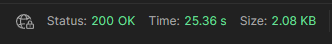
\includegraphics[width=0.5\textwidth]{resources/ch4/time/1-postman.png}
	\caption{\textit{Response time} dari Postman untuk kasus SI1}
	\label{time_p_1}
\end{figure}

\begin{figure}[!htb]
	\centering
	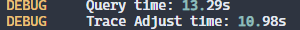
\includegraphics[width=0.5\textwidth]{resources/ch4/time/1-log.png}
	\caption{Pencatatan waktu fungsi kasus SI1}
	\label{time_l_1}
\end{figure}



\subsection{Analisis Hasil Pengujian}
Dari semua kasus pengujian, hasil yang didapatkan dari pengujian akan bergantung pada nilai signifikan yang digunakan untuk menguji masing-masing kasus. Terdapat 3 nilai signifikan yang penulis gunakan untuk melakukan pengujian yaitu 0,1, 0,005, dan 0,001 dengan maksud menguji sensitivitas dari algoritma pendeteksian regresi diberikan nilai signifikan yang berbeda-beda. Hasilnya adalah pengujian dengan nilai signifikan 0,1 berhasil mendeteksi dan menganalisis penyebab regresi dengan benar pada semua kasus uji, namun pada pengujian dengan nilai signifikan 0,05 dan 0,001 kasus SI1 tidak terdeteksi sebagai regresi.

Gambar \ref{result_log_1} menunjukkan \textit{log} yang didapatkan dari kasus SI1 dengan nilai signifikan 0,05.


Dari hasil pengujian, pada level signifikan 0,01 semua kasus regresi dapat dideteksi 

Dari tujuh kasus uji, kasus SI1 sampai SI7, yang menyimulasikan terjadinya regresi akibat perubahan di level kode, hanya satu kasus, yaitu kasus SI1, yang regresi tidak dapat terdeteteksi oleh PRA Engine. Selebihnya, dari enam kasus lainnya, PRA Engine dapat mendeteksi terjadinya regresi dan juga dapat menentukan kandidat operasi sumber terjadinya regresi dengan menghitung selisih \textit{latency} antara data \textit{trace} \textit{baseline} dan periodikal. 

\begin{figure}[!htb]
	\centering
	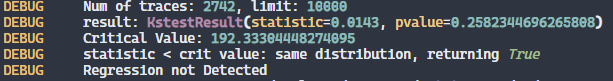
\includegraphics[width=1\textwidth]{resources/ch4/log/1-log.png}
	\caption{\textit{Log} hasil pengujian kasus SI1 dengan alpha 0,05}
	\label{result_log_1}
\end{figure}

Gambar \ref{result_log_1} merupakan \textit{log} yang didapatkan dari kasus SI1 yang menampilkan hasil tes statistik K-S. Nilai \texttt{p-value} yang didapatkan dari hasil tes lebih besar dari nilai signifikan yaitu 0.05 dan juga nilai \texttt{statistic} lebih kecil dari nilai \texttt{critical value} sehingga hipotesis $h_{0}$ tidak dapat ditolak dan PRA Engine menginterpretasikan bahwa data \textit{latency} dari kasus SI1 berasal dari distribusi yang sama dengan data \textit{latency} \textit{baseline}. 

Dari analisis hasil kasus SI1 dapat terlihat bahwa algoritma tidak dapat mendeteksi terjadinya regresi jika tidak terdapat perbedaan signifikan antara kedua sampel data seperti pada kasus SI1 yang hanya menyimulasikan penambahan \textit{latency} sebesar 100ms pada satu buah operasi. Sementara pada kasus selanjutnya, yaitu kasus SI2 dengan penambahan \textit{latency} sebesar 250ms, PRA Engine dapat mendeteksi bahwa data \textit{latency} periodikal berasal dari distribusi yang berbeda dengan data \textit{latency} \textit{baseline} sehingga PRA Engine dapat mendeteksi terjadinya regresi.

Sementara pada kasus-kasus yang menyimulasikan perubahan dari eksternal, yaitu kasus SE1 sampai SE4, PRA Engine juga dapat mendeteksi terjadinya regresi karena algoritma dapat menentukan bahwa data \textit{latency} pada kasus-kasus tersebut berasal dari distribusi yang berbeda dari data \textit{latency} \textit{baseline}.

Dapat disimpulkan bahwa algoritma belum dapat menentukan apakah regresi yang terjadi diakibatkan oleh perubahan yang terjadi pada level aplikasi ataupun perubahan yang terjadi di luar aplikasi seperti peningkatan jumlah pengguna ataupun peningkatan \textit{load} pada sebagian operasi. Namun jika dari analisis \textit{critical path} dapat terlihat selisih \textit{latency} dari operasi yang melebihi \textit{threshold} tertentu dapat menjadi indikasi bahwa regresi yang terjadi diakibatkan oleh perubahan di level aplikasi. Sebaliknya, jika analisis \textit{critical path} tidak dapat menentukan operasi yang menjadi kandidat penyebab regresi karena selisihnya tidak lebih besar daripada \textit{threshold}, seperti yang terlihat pada gambar \ref{result_json_8}, maka dapat menjadi indikasi bahwa regresi yang terdeteksi diakibatkan oleh perubahan yang disebabkan oleh faktor eksternal.

%----------------------------------------------------------------%

% Daftar pustaka
% Bibliography to Daftar Pustaka
\renewcommand{\bibname}{Daftar Pustaka}
\clearpage
\phantomsection
\pagenumbering{roman}
\setcounter{page}{\thesavepage}
\bibliography{references}
\bibliographystyle{apalike}


\end{document}
